% toolsoftrade/toolsoftrade.tex

\QuickQuizChapter{chp:Tools of the Trade}{Tools of the Trade}
%
\Epigraph{You are only as good as your tools, and your tools are only
	  as good as you are.}{\emph{Unknown}}

이 챕터에서는 리눅스와 유사한 운영체제에서 돌아가는 어플리케이션에서 사용할 수
있는 것들에 집중해서 몇몇 기본적인 병렬 프로그래밍 도구를 소개합니다.
Section~\ref{sec:toolsoftrade:Scripting Languages} 는 스크립트 언어로 시작을
하고,
Section~\ref{sec:toolsoftrade:POSIX Multiprocessing} 에서는 POSIX API 로
지원되는 멀티 프로세스 병렬성을 설명하고 POSIX 쓰레드를 다뤄보고,
Section~\ref{sec:toolsoftrade:Alternatives to POSIX Operations}
는 다른 환경들에서의 비슷한 오퍼레이션들을 선보이며, 마지막으로,
Section~\ref{sec:toolsoftrade:The Right Tool for the Job: How to Choose?}
에서는 일을 완료하기 위해 어떤 도구를 골라야 할지 선택을 도와드립니다.
\iffalse

This chapter provides a brief introduction to some basic tools of the
parallel-programming trade, focusing mainly on those available to
user applications running on operating systems similar to Linux.
Section~\ref{sec:toolsoftrade:Scripting Languages} begins with
scripting languages,
Section~\ref{sec:toolsoftrade:POSIX Multiprocessing}
describes the multi-process parallelism supported by the POSIX API and
touches on POSIX threads,
Section~\ref{sec:toolsoftrade:Alternatives to POSIX Operations}
presents analogous operations in other environments, and finally,
Section~\ref{sec:toolsoftrade:The Right Tool for the Job: How to Choose?}
helps to choose the tool that will get the job done.
\fi

\QuickQuiz{}
	이것들을 도구라고 하셨나요???
	제게 이것들은 도구라기보다는 낮은 단계의 동기화 기능들처럼 보이는데요!
	\iffalse

	You call these tools???
	They look more like low-level synchronization primitives to me!
	\fi
\QuickQuizAnswer{
	그것들은 실제로 낮은 단계의 동기화 기능들이기 때문에 그렇게 보입니다.
	하지만 또한, 그것들은 실제로 낮은 단계의 동시성 있는 소프트웨어를
	만드는데 사용되는 기본적인 도구들입니다.
	\iffalse

	They look that way because they are in fact low-level synchronization
	primitives.
	But as such, they are in fact the fundamental tools for building
	low-level concurrent software.
	\fi
} \QuickQuizEnd

이 챕터는 간략한 소개만을 제공한다는 점을 기억해 두세요.
더 자세한 내용은 (특히 인터넷에서)인용된 참조 목록들에서 볼 수 있으며, 이
도구들을 어떻게 사용하는게 최선인지는 뒤의 챕터들에서 설명합니다.
\iffalse

Please note that this chapter provides but a brief introduction.
More detail is available from the references cited (and especially
from Internet), and more information
on how best to use these tools will be provided in later chapters.
\fi

\section{Scripting Languages}
\label{sec:toolsoftrade:Scripting Languages}

리눅스 셸 스크립트 언어들은 병렬성을 관리하는 간단하지만 효과적인 방법들을
제공합니다.
예를 들어, 당신이 \co{compute_it} 이라는 이름의 프로그램을 가지고 있는데 두개의
다른 인자들로 두번 수행해야 한다고 생각해 봅시다.
이는 UNIX 셸 스크립트를 사용해서 다음과 같이 이뤄질 수 있습니다:
\iffalse

The Linux shell scripting languages provide simple but effective ways
of managing parallelism.
For example, suppose that you had a program \co{compute_it}
that you needed to run twice with two different sets of arguments.
This can be accomplished using UNIX shell scripting as follows:
\fi

\input{CodeSamples/toolsoftrade/parallel@compute_it.fcv}

\begin{figure}[tb]
\centering
\resizebox{3in}{!}{\includegraphics{toolsoftrade/shellparallel}}
\caption{Execution Diagram for Parallel Shell Execution}
\label{fig:toolsoftrade:Execution Diagram for Parallel Shell Execution}
\end{figure}

라인~1 과~2 는 이 프로그램의 인스턴스를 두개 실행시키고, 각 인스턴스의 결과물을
두개의 별개의 파일에 집어넣는데, \co{&} 문자는 셸이 그 두 프로그램 인스턴스를
백그라운드에서 실행하도록 합니다.
라인~3 은 두개의 인스턴스 모두가 종료되길 기다리고, 라인~4 와 5 에서는 그들의
결과값을 화면에 출력합니다.
실행 흐름은
Figure~\ref{fig:toolsoftrade:Execution Diagram for Parallel Shell Execution}
에 나타낸 대로입니다:
\co{compute_it} 의 두개의 인스턴스는 병렬적으로 수행되고, \co{wait} 은 두개
인스턴스 모두가 완료된 뒤에 완료되며, 그 뒤에 \co{cat} 의 두개의 인스턴스가
순차적으로 수행됩니다.
\iffalse

% TODO: apply
\begin{lineref}[ln:toolsoftrade:parallel:compute_it]
Lines~\lnref{comp1} and~\lnref{comp2} launch two instances of this
program, redirecting their
output to two separate files, with the \co{&} character directing the
shell to run the two instances of the program in the background.
Line~\lnref{wait} waits for both instances to complete, and
lines~\lnref{cat1} and~\lnref{cat2}
display their output.
\end{lineref}
The resulting execution is as shown in
Figure~\ref{fig:toolsoftrade:Execution Diagram for Parallel Shell Execution}:
the two instances of \co{compute_it} execute in parallel,
\co{wait} completes after both of them do, and then the two instances
of \co{cat} execute sequentially.
% @@@ Maui scheduler, load balancing, BOINC, and so on.
% @@@ Diagram showing parallel execution.
\fi

\QuickQuiz{}
	하지만 이 간단한 셸 스크립트는 \emph{진짜} 병렬 프로그램이 아니잖아요!
	왜 이런 별거아닌 걸 신경쓰는거죠???
	\iffalse

	But this silly shell script isn't a \emph{real} parallel program!
	Why bother with such trivia???
	\fi
\QuickQuizAnswer{
	당신은 \emph{결코} 이 간단한 것을 잊지 않아야 하기 때문입니다!

	이 책의 제목이 ``Is Parallel Programming Hard, And, If So, What Can You
	Do About It?'' 이란 걸 마음에 새겨 두십시오.
	당신이 할 수 있는 가장 효과적인 일은 그 간단한 것을 잊지 않도록 하는
	것입니다!
	무엇보다, 당신이 그 어려운 병렬 프로그래밍을 하기로 선택했다면, 당신의
	선택이니, 당신 자신 외의 누구에게도 불평 할 수 없습니다.
	\iffalse

	Because you should \emph{never} forget the simple stuff!

	Please keep in mind that the title of this book is
	``Is Parallel Programming Hard, And, If So, What Can You Do About It?''.
	One of the most effective things you can do about it is to
	avoid forgetting the simple stuff!
	After all, if you choose to do parallel programming the hard
	way, you have no one but yourself to blame.
	\fi
} \QuickQuizEnd

\QuickQuiz{}
	병렬 셸 스크립트를 작성하는 좀 더 간단한 방법은 없나요?
	만약 있다면, 어떻게 하나요? 없다면, 왜 없죠?
	\iffalse

	Is there a simpler way to create a parallel shell script?
	If so, how?  If not, why not?
	\fi
\QuickQuizAnswer{
	가장 직관적인 방법은 셸 파이프라인입니다:
	\iffalse

	One straightforward approach is the shell pipeline:
	\fi

\begin{minipage}[t]{\columnwidth}
\vspace{0.1ex}
\small
\begin{verbatim}
grep $pattern1 | sed -e 's/a/b/' | sort
\end{verbatim}
\vspace{0.1ex}
\end{minipage}
	충분히 커다란 입력 파일에 대해서, \co{grep} 의 패턴 매칭, \co{sed} 의
	수정과 \co{sort} 의 입력물 처리는 병렬적으로 수행될 겁니다.
	\path{parallel.sh} 파일에 셸 스크립트 병렬성과 파이프라인에 대한 데모가
	있습니다.
	\iffalse

	For a sufficiently large input file,
	\co{grep} will pattern-match in parallel with \co{sed}
	editing and with the input processing of \co{sort}.
	See the file \path{parallel.sh} for a demonstration of
	shell-script parallelism and pipelining.
	\fi
} \QuickQuizEnd

다른 예로, 소프트웨어 빌드 스크립트 언어인 \co{make} 는 얼마나 많은 병렬성이
해당 빌드 작업에 주어져야 하는지 결정하는 \co{-j} 옵션을 제공합니다.
예를 들어, 리눅스 커널을 빌드할 때 \co{make -j4} 명령을 입력하는 것은 최대
4개의 병렬 컴파일이 동시에 수행될 것을 말합니다.

이런 간단한 예가 당신에게 병렬 프로그래밍이 항상 복잡하거나 어려울 필요는
없음을 납득시켜 주길 바랍니다.
\iffalse

For another example, the \co{make} software-build scripting language
provides a \co{-j} option that specifies how much parallelism should be
introduced into the build process.
For example, typing \co{make -j4} when building a Linux kernel
specifies that up to four parallel compiles be carried out concurrently.

It is hoped that these simple examples convince you that parallel
programming need not always be complex or difficult.
\fi

\QuickQuiz{}
	하지만 스크립트 기반 병렬 프로그래밍이 그렇게 쉽다면, 왜 다른 것들을
	신경쓰는거죠?
	\iffalse

	But if script-based parallel programming is so easy, why
	bother with anything else?
	\fi
\QuickQuizAnswer{
	사실 오늘날 사용되는 병렬 프로그램들의 매우 많은 부분들이 스크립트에
	기반합니다.
	하지만, 스크립트 기반 병렬성은 한계점도 지니고 있습니다:
	\iffalse

	In fact, it is quite likely that a very large fraction of
	parallel programs in use today are script-based.
	However, script-based parallelism does have its limitations:
	\fi
	\begin{enumerate}
	\item	새 프로세스의 생성은 보통 비싼 시스템콜인 \co{fork()} 와
		\co{exec()} 를 포함하기 때문에 상당히 무거운 작업입니다.
	\item	파이프라이닝을 포함해서 데이터의 공유는 일반적으로 비싼 file
		I/O 를 포함합니다.
	\item	스크립트에서 믿고 쓸 수 있는 동기화 기본 도구들 역시 일반적으로
		비싼 file I/O 를 포함합니다.
	\item	스크립트 언어들은 많은 경우 너무 느립니다만, 더 낮은 단계의
		프로그래밍 언어로 쓰여진, 오랫동안 수행되는 프로그램의 수행을
		조정할 때에는 많은 경우 상당히 유용합니다.
	\iffalse

	\item	Creation of new processes is usually quite heavyweight,
		involving the expensive \co{fork()} and \co{exec()}
		system calls.
	\item	Sharing of data, including pipelining, typically involves
		expensive file I/O.
	\item	The reliable synchronization primitives available to
		scripts also typically involve expensive file I/O.
	\item	Scripting languages are often too slow, but are often
		quite useful when coordinating execution of long-running
		programs written in lower-level programming languages.
	\fi
	\end{enumerate}
	이런 제한점들은 스크립트 기반 병렬성이 coarse-grained 병렬성을 사용하고
	각 일의 단위들은 최소 수십 밀리세컨드, 그리고 가능하다면 그보다도 훨씬
	긴 시간을 가질 것을 요구합니다.
	\iffalse

	These limitations require that script-based parallelism use
	coarse-grained parallelism, with each unit of work having
	execution time of at least tens of milliseconds, and preferably
	much longer.
	\fi

	finer-grained 병렬성을 필요로 하는 작업들은 그 작업의 문제가
	coarse-grained 형태로 표현될 수는 없을지 좀 고민해 보도록 추천됩니다.
	만약 불가능하다면, Section~\ref{sec:toolsoftrade:POSIX Multiprocessing}
	에서 다루는 것과 같은 다른 병렬 프로그래밍 환경을 고려해 봐야 합니다.
	\iffalse

	Those requiring finer-grained parallelism are well advised to
	think hard about their problem to see if it can be expressed
	in a coarse-grained form.
	If not, they should consider using other parallel-programming
	environments, such as those discussed in
	Section~\ref{sec:toolsoftrade:POSIX Multiprocessing}.
	\fi
} \QuickQuizEnd

\section{POSIX Multiprocessing}
\label{sec:toolsoftrade:POSIX Multiprocessing}

이 섹션에서는 사용 가능하고 널리 구현되어 있는,
pthread~\cite{OpenGroup1997pthreads} 를 포함해 POSIX 환경의 겉부분을
알아봅니다.
Section~\ref{sec:toolsoftrade:POSIX Process Creation and Destruction}
에서는 POSIX \co{fork()} 와 관련된 기능들을 살짝 훑어보고,
Section~\ref{sec:toolsoftrade:POSIX Thread Creation and Destruction}
에서는 쓰레드 생성과 소멸에 대해 간단히 알아본 후,
Section~\ref{sec:toolsoftrade:POSIX Locking} 에서는 POSIX 락킹에 대한 짧은
개요를 제공할 예정이며, 마지막으로,
Section~\ref{sec:toolsoftrade:POSIX Reader-Writer Locking} 에서 여러 쓰레드에
의해 읽히고 가끔만 갱신되는 데이터에 대해 사용되곤 하는 특정한 락에 대해
설명합니다.
\iffalse

This section scratches the surface of the
POSIX environment, including pthreads~\cite{OpenGroup1997pthreads},
as this environment is readily available and widely implemented.
Section~\ref{sec:toolsoftrade:POSIX Process Creation and Destruction}
provides a glimpse of the POSIX \co{fork()} and related primitives,
Section~\ref{sec:toolsoftrade:POSIX Thread Creation and Destruction}
touches on thread creation and destruction,
Section~\ref{sec:toolsoftrade:POSIX Locking} gives a brief overview
of POSIX locking, and, finally,
Section~\ref{sec:toolsoftrade:POSIX Reader-Writer Locking} describes a
specific lock which can be used for data that is read by many threads and only
occasionally updated.
\fi

\subsection{POSIX Process Creation and Destruction}
\label{sec:toolsoftrade:POSIX Process Creation and Destruction}

프로세스는 \co{fork()} 를 통해 생성되고, \co{kill()} 를 통해 소멸 당할 수도,
스스로 \co{exit()} 를 통해 소멸될 수도 있습니다.
\co{fork()} 를 실행하는 프로세스는 새로 생성되는 프로세스의 ``부모'' 라고
불리웁니다.
부모는 \co{wait()} 를 통해 자기 자식들을 기다릴 수도 있습니다.
\iffalse

Processes are created using the \co{fork()} primitive, they may
be destroyed using the \co{kill()} primitive, they may destroy
themselves using the \co{exit()} primitive.
A process executing a \co{fork()} primitive is said to be the ``parent''
of the newly created process.
A parent may wait on its children using the \co{wait()} primitive.
\fi

이 섹션의 예제들은 상당히 간단한 것들이란 점을 기억해 두시기 바랍니다.
이 간단한 도구들을 사용하는 실제 어플리케이션들은 시그널, 파일 디스크립터,
공유된 메모리 조각, 그리고 또다른 많은 자원들을 제어해야 할 수도 있을 겁니다.
또한, 어떤 어플리케이션은 어떤 자식 프로세스가 종료되었을 때 특별한 행동을
취해야 할 수도 있고, 또한 자식 프로세스가 어떤 이유로 종료되었는지에 대해서도
신경써야 할 수 있습니다.
이렇게 신경써야 하는 부분들은 물론 코드에 상당한 복잡도를 추가할 수 있습니다.
더 많은 내용을 위해서는, 해당 주제에 대한
교재들~\cite{WRichardStevens1992,StewartWeiss2013UNIX} 을 보시기 바랍니다.
\iffalse

Please note that the examples in this section are quite simple.
Real-world applications using these primitives might need to manipulate
signals, file descriptors, shared memory segments, and any number of
other resources.
In addition, some applications need to take specific actions if a given
child terminates, and might also need to be concerned with the reason
that the child terminated.
These concerns can of course add substantial complexity to the code.
For more information, see any of a number of textbooks on the
subject~\cite{WRichardStevens1992,StewartWeiss2013UNIX}.
\fi

\begin{listing}[tbp]
\begin{linelabel}[ln:toolsoftrade:forkjoin:main]
\begin{VerbatimL}[commandchars=\%\[\]]
pid = fork();%lnlbl[fork]
if (pid == 0) {%lnlbl[if]
	/* child */%lnlbl[child]
} else if (pid < 0) {%lnlbl[else]
	/* parent, upon error */%lnlbl[errora]
	perror("fork");
	exit(EXIT_FAILURE);%lnlbl[errorb]
} else {
	/* parent, pid == child ID */%lnlbl[parent]
}
\end{VerbatimL}
\end{linelabel}
\caption{Using the \tco{fork()} Primitive}
\label{lst:toolsoftrade:Using the fork() Primitive}
\end{listing}

\begin{lineref}[ln:toolsoftrade:forkjoin:main]
\co{fork()} 가 성공하면, \co{fork()}는 한번은 부모에게, 또한번은 자식에게 두번
리턴합니다.
\co{fork()} 가 리턴하는 값은
Listing~\ref{lst:toolsoftrade:Using the fork() Primitive}
(\path{forkjoin.c}) 에 보여진 것처럼 호출자가 그 차이를 알 수 있게 합니다.
라인~\lnref{fork} 는\co{fork()} 함수를 실행하고, 그 리턴값을 지역 변수 \co{pid}
에 저장합니다.
라인~\lnref{if} 에서는 \co{pid} 가 0인지 체크하는데, 만약 맞다면 자신은 자식
프로세스라는 뜻이며, 이 경우 코드 실행은 라인~\lnref{child} 으로 이어집니다.
앞서 이야기 했듯, 자식 프로세스는 \co{exit()} 기능을 통해 종료될 수 있습니다.
만약 \co{fork()} 리턴값이 0이 아니어서 자신이 부모 프로세스라면,
라인~\lnref{else} 에서 얻은 \co{fork()} 리턴값을 가지고 에러가 있었는지
확인하고, 에러가 있었다면 라인~\lnref{errora}-\lnref{errorb} 에서 에러를
화면에 출력하고 종료합니다.
그렇지 않고 \co{fork()} 가 성공적으로 수행되었다면, 자식 프로세스의 프로세스 ID
값을 가지고 있는 변수 \co{pid} 와 함께 라인~\lnref{parent}로 넘어갑니다.
\end{lineref}
\iffalse

\begin{lineref}[ln:toolsoftrade:forkjoin:main]
If \co{fork()} succeeds, it returns twice, once for the parent
and again for the child.
The value returned from \co{fork()} allows the caller to tell
the difference, as shown in
Listing~\ref{lst:toolsoftrade:Using the fork() Primitive}
(\path{forkjoin.c}).
Line~\lnref{fork} executes the \co{fork()} primitive, and saves
its return value in local variable \co{pid}.
Line~\lnref{if} checks to see if \co{pid} is zero, in which case,
this is the child, which continues on to execute line~\lnref{child}.
As noted earlier, the child may terminate via the \co{exit()} primitive.
Otherwise, this is the parent, which checks for an error return from
the \co{fork()} primitive on line~\lnref{else}, and prints an error
and exits on lines~\lnref{errora}-\lnref{errorb} if so.
Otherwise, the \co{fork()} has executed successfully, and the parent
therefore executes line~\lnref{parent} with the variable \co{pid}
containing the process ID of the child.
\end{lineref}
\fi

\begin{listing}[tbp]
\input{CodeSamples/api-pthreads/api-pthreads@waitall.fcv}
\caption{Using the \tco{wait()} Primitive}
\label{lst:toolsoftrade:Using the wait() Primitive}
\end{listing}

\begin{lineref}[ln:api-pthreads:api-pthreads:waitall]
부모 프로세스는 자식 프로세스가 완료될 때까지 \co{wait()} 함수를 이용해 기다릴
수도 있습니다.
하지만, 하나의 \co{wait()} 호출은 오로지 한개의 자식 프로세스만 기다리기
때문에, 이 함수의 사용은 셸 스크립트에서의 같은 이름의 기능을 사용할 때보다 좀
더 복잡합니다.
그래서
Listing~\ref{lst:toolsoftrade:Using the wait() Primitive}
(\path{api-pthread.h})
에서 보여진, 셸 스크립트 에서의 \co{wait} 명령과 유사한 의미를 가진,
\co{waitall()} 함수와 비슷한 함수로 \co{wait()} 를 감싸는게 일반적입니다.
라인~\lnref{loopa}-\lnref{loopb} 에서의 루프의 각 패스에서는 한개 자식
프로세스를 기다립니다.
라인~\lnref{wait} 에서는 \co{wait()} 함수를 호출하는데, 이 함수는 자식 프로세스
하나가 종료될 때까지 부모 프로세스를 블록시키고, 자식 프로세스가 종료된 후 자식
프로세스의 프로세스 ID 를 리턴합니다.
만약 프로세스 ID 가 아니라 $-1$ 이 리턴된다면, 이는 \co{wait()} 함수가 자식
프로세스를 기다릴 수 없었음을 의미합니다.
만약 그렇다면, 라인~\lnref{ECHILD} 에서 errno 가 \co{ECHILD} 로 되었는지 여부를
체크하는데, 만약 그렇다면 더이상 자식 프로세스가 존재하지 않는다는 의미로, 이
때엔 라인~\lnref{break} 에서 루프를 빠져나옵니다.
그렇지 않다면, 라인~\lnref{perror} 과~\lnref{exit} 에서 에러를 출력하고
종료합니다.
\end{lineref}
\iffalse

\begin{lineref}[ln:api-pthreads:api-pthreads:waitall]
The parent process may use the \co{wait()} primitive to wait for its children
to complete.
However, use of this primitive is a bit more complicated than its shell-script
counterpart, as each invocation of \co{wait()} waits for but one child
process.
It is therefore customary to wrap \co{wait()} into a function similar
to the \co{waitall()} function shown in
Listing~\ref{lst:toolsoftrade:Using the wait() Primitive}
(\path{api-pthread.h}),
with this \co{waitall()} function having semantics similar to the
shell-script \co{wait} command.
Each pass through the loop spanning lines~\lnref{loopa}-\lnref{loopb}
waits on one child process.
Line~\lnref{wait} invokes the \co{wait()} primitive, which blocks
until a child process exits, and returns that child's process ID.
If the process ID is instead $-1$, this indicates that the \co{wait()}
primitive was unable to wait on a child.
If so, line~\lnref{ECHILD} checks for the \co{ECHILD} errno, which
indicates that there are no more child processes, so that
line~\lnref{break} exits the loop.
Otherwise, lines~\lnref{perror} and~\lnref{exit} print an error and exit.
\end{lineref}
\fi

\QuickQuiz{}
	왜 이 \co{wait()} 함수는 그렇게 복잡해야만 하는거죠?
	왜 그냥 셸 스크립트의 \co{wait} 같이 동작하도록 만들지 않는 거예요?
	\iffalse

	Why does this \co{wait()} primitive need to be so complicated?
	Why not just make it work like the shell-script \co{wait} does?
	\fi
\QuickQuizAnswer{
	일부 병렬 어플리케이션은 특정 자식 프로세스가 끝났을 때 특별한 행동을
	취해야 해서, 각 자식 프로세스에 대해 개별적으로 대기를 할 필요가 있을
	수 있습니다.
	또한, 일부 병렬 어플리케이션들은 자식 프로세스가 종료된 이유를 알
	필요도 있습니다.
	Listing~\ref{lst:toolsoftrade:Using the wait() Primitive} 에서 본
	것처럼, \co{wait()} 함수를 가지고 \co{waitall()} 함수를 만드는 건
	어렵지 않습니다만 그 반대는 불가능하겠지요.
	한번 특정 자식 프로세스에 대한 정보를 잃어버리면, 되돌이킬 수 없습니다.
	\iffalse

	Some parallel applications need to take special action when
	specific children exit, and therefore need to wait for each
	child individually.
	In addition, some parallel applications need to detect the
	reason that the child died.
	As we saw in Listing~\ref{lst:toolsoftrade:Using the wait() Primitive},
	it is not hard to build a \co{waitall()} function out of
	the \co{wait()} function, but it would be impossible to
	do the reverse.
	Once the information about a specific child is lost, it is lost.
	\fi
} \QuickQuizEnd

\begin{listing}[tbp]
\input{CodeSamples/toolsoftrade/forkjoinvar@main.fcv}
\caption{Processes Created Via \tco{fork()} Do Not Share Memory}
\label{lst:toolsoftrade:Processes Created Via fork() Do Not Share Memory}
\end{listing}

\begin{lineref}[ln:toolsoftrade:forkjoinvar:main]
부모와 자식 프로세스가 메모리를 공유하지 \emph{않는}다는 점은 매우 중요하므로
반드시 기억해야 합니다.
이는
Listing~\ref{lst:toolsoftrade:Processes Created Via fork() Do Not Share Memory}
(\path{forkjoinvar.c}) 의 프로그램으로 보여지는데, 자식 프로세스는
라인~\lnref{setx} 에서 전역 변수 \co{x} 를 1로 만들고 라인~\lnref{print:c} 에서
메세지를 프린트한 후, 라인~\lnref{exit:s} 에서 종료합니다.
부모는 라인~\lnref{waitall} 에서 실행 흐름을 이어서 자식 프로세스를 기다리고
라인~\lnref{print:p} 에서 변수 \co{x} 의 값을 보지만 여전히 그 값은 0입니다.
따라서 이 프로그램의 출력은 다음과 같습니다:
\end{lineref}
\iffalse

\begin{lineref}[ln:toolsoftrade:forkjoinvar:main]
It is critically important to note that the parent and child do \emph{not}
share memory.
This is illustrated by the program shown in
Listing~\ref{lst:toolsoftrade:Processes Created Via fork() Do Not Share Memory}
(\path{forkjoinvar.c}),
in which the child sets a global variable \co{x} to 1 on line~\lnref{setx},
prints a message on line~\lnref{print:c}, and exits on line~\lnref{exit:s}.
The parent continues at line~\lnref{waitall}, where it waits on the child,
and on line~\lnref{print:p} finds that its copy of the variable \co{x} is
still zero. The output is thus as follows:
\end{lineref}
\fi

\begin{VerbatimU}
Child process set x=1
Parent process sees x=0
\end{VerbatimU}

\QuickQuiz{}
	여기서 이야기한 것 외에도 \co{fork()} 와 \co{wait()} 에 대해 이야기할
	것들이 많지 않나요?
	\iffalse

	Isn't there a lot more to \co{fork()} and \co{wait()}
	than discussed here?
	\fi
\QuickQuizAnswer{
	맞습니다, 그리고 그리고 이 섹션은 나중에 (UNIX 파이프, TCP/IP, 그리고
	공유 파일 I/O 같은) 메세징 기능과 (\co{mmap()} 과 \co{shmget()} 같은)
	메모리 매핑 기능에 대한 논의를 포함하도록 확장될 수도 있을 겁니다.
	그 전까지는, 이런 기능들에 대해 훨씬 자세하게 설명하는 다른 교재들이
	많이 있고, 정말 잘 알고 싶다면 man 페이지(역주: UNIX 커맨드
	\co{man})나, 이런 기능을 사용하는 현존 병렬 어플리케이션들, 또는 리눅스
	커널 구현의 소스 코드를 참고해도 될 것입니다.

	Listing~\ref{lst:toolsoftrade:Processes Created Via fork() Do Not Share Memory}
	의 부모 프로세스는 자식 프로세스가 종료될 때까지 자신의 \co{printf()}
	를 위해 기다리고 있다는 것을 기억해 둘 필요가 있습니다.
	\co{printf()} 의 buffered I/O 를 같은 파일에 대해 여러 프로세스에서
	동시적으로 사용하는 것은 일반적이지 않고, 그러지 않는게 최선입니다.
	정말로 동시적으로 buffered I/O 를 해야만 한다면, 여러분 OS 의 문서를
	참고하세요.
	UNIX/Linux 시스템에서는 Stewart Weiss 의 강의 노트가
	예제~\cite{StewartWeiss2013UNIX} 와 함께 좋은 소개를 제공합니다.
	\iffalse

	Indeed there is, and
	it is quite possible that this section will be expanded in
	future versions to include messaging features (such as UNIX
	pipes, TCP/IP, and shared file I/O) and memory mapping
	(such as \co{mmap()} and \co{shmget()}).
	In the meantime, there are any number of textbooks that cover
	these primitives in great detail,
	and the truly motivated can read manpages, existing parallel
	applications using these primitives, as well as the
	source code of the Linux-kernel implementations themselves.

	It is important to note that the parent process in
	Listing~\ref{lst:toolsoftrade:Processes Created Via fork() Do Not Share Memory}
	waits until after the child terminates to do its \co{printf()}.
	Using \co{printf()}'s buffered I/O concurrently to the same file
	from multiple processes is non-trivial, and is best avoided.
	If you really need to do concurrent buffered I/O,
	consult the documentation for your OS.
	For UNIX/Linux systems, Stewart Weiss's lecture notes provide
	a good introduction with informative
	examples~\cite{StewartWeiss2013UNIX}.
	\fi
} \QuickQuizEnd

가장 잘게 크리티컬 섹션을 쪼갠 병렬성은 공유 메모리를 필요로 하며, 이는
Section~\ref{sec:toolsoftrade:POSIX Thread Creation and Destruction} 에서
다룹니다.
하지만, 공유 메모리 병렬성은 fork-join 병렬성에 비해 상당히 복잡할 수 있습니다.
\iffalse

The finest-grained parallelism requires shared memory, and
this is covered in
Section~\ref{sec:toolsoftrade:POSIX Thread Creation and Destruction}.
That said, shared-memory parallelism can be significantly more complex
than fork-join parallelism.
\fi

\subsection{POSIX Thread Creation and Destruction}
\label{sec:toolsoftrade:POSIX Thread Creation and Destruction}

프로세스 내에서 쓰레드를 생성하려면
Listing~\ref{lst:toolsoftrade:Threads Created Via pthread-create() Share Memory}
(\path{pcreate.c}) 의 라인~15 와~16 에 보인 것처럼 \co{pthread_create()} 함수를
호출해야 합니다.
첫번째 인자는 \co{pthread_t} 타입 변수로의 포인터로, 해당 쓰레드의 ID 를
저장하게 되며, 예제에서는 \co{NULL} 값을 준 두번째 인자는 필요하면 추가하게
되는 \co{pthread_attr_t} 타입 변수로의 포인터이며, 세번째 인자는 새로 생성된
쓰레드에 의해 호출될 함수(이 경우, \co{mythread()}) 이고, 여기선 \co{NULL} 을
준 마지막 인자는 \co{mythread} 에게 전달될 인자입니다.
\iffalse

% TODO: Apply
\begin{lineref}[ln:toolsoftrade:pcreate:mythread]
To create a thread within an existing process, invoke the
\co{pthread_create()} primitive, for example, as shown on
lines~\lnref{create:a} and~\lnref{create:b} of
Listing~\ref{lst:toolsoftrade:Threads Created Via pthread-create() Share Memory}
(\path{pcreate.c}).
The first argument is a pointer to a \co{pthread_t} in which to store the
ID of the thread to be created, the second \co{NULL} argument is a pointer
to an optional \co{pthread_attr_t}, the third argument is the function
(in this case, \co{mythread()})
that is to be invoked by the new thread, and the last \co{NULL} argument
is the argument that will be passed to \co{mythread}.
\end{lineref}
\fi

\begin{listing}[tbp]
\input{CodeSamples/toolsoftrade/pcreate@mythread.fcv}
\caption{Threads Created Via \tco{pthread_create()} Share Memory}
\label{lst:toolsoftrade:Threads Created Via pthread-create() Share Memory}
\end{listing}

이 예제에서, \co{mythread()} 는 단순히 리턴하지만, 대신 \co{pthread_exit()} 를
사용할 수도 있습니다.
\iffalse

In this example, \co{mythread()} simply returns, but it could instead
call \co{pthread_exit()}.
\fi

\QuickQuiz{}
	Listing~\ref{lst:toolsoftrade:Threads Created Via pthread-create() Share Memory}
	의 \co{mythread()} 함수가 그냥 리턴해도 된다면, 왜 \co{pthread_exit()}
	를 신경쓰는 거죠?
	\iffalse

	If the \co{mythread()} function in
	Listing~\ref{lst:toolsoftrade:Threads Created Via pthread-create() Share Memory}
	can simply return, why bother with \co{pthread_exit()}?
	\fi
\QuickQuizAnswer{
	이 간단한 예제에서는 \co{pthread_exit()} 를 신경 쓸 이유가 없는게
	맞습니다.
	하지만, \co{mythread()} 가 별도로 컴파일된 다른 함수를 호출하는 경우를
	생각해 봅시다.
	그런 경우, \co{pthread_exit()} 는 이런 다른 함수들에서도 별도의 다른
	에러들을 리턴하거나 해서 실행 흐름을 \co{mythread()} 에 되돌릴 필요
	없이 곧바로 쓰레드의 실행을 종료시킬 수 있게 합니다.
	\iffalse

	In this simple example, there is no reason whatsoever.
	However, imagine a more complex example, where \co{mythread()}
	invokes other functions, possibly separately compiled.
	In such a case, \co{pthread_exit()} allows these other functions
	to end the thread's execution without having to pass some sort
	of error return all the way back up to \co{mythread()}.
	\fi
} \QuickQuizEnd

\begin{lineref}[ln:toolsoftrade:pcreate:mythread]
라인~\lnref{join} 에 있는 \co{pthread_join()} 함수는 fork-join 에서의
\co{wait()} 함수와 유사합니다.
이 함수는 \co{tid} 변수로 명시된 쓰레드가 \co{pthread_exit()} 함수를 통해서,
또는 쓰레드의 탑 레벨 함수가 리턴을 해서 실행을 완료할 때까지 기다립니다.
쓰레드의 종료 값은 \co{pthread_join()} 함수에 두번째 인자로 넘겨진 포인터를
통해 저장됩니다.
쓰레드의 종료 값은 쓰레드가 어떻게 종료되었는지에 따라 다른데,
\co{pthread_exit()} 함수에 넘겨진 값이거나 쓰레드의 탑 레벨 함수에서 리턴한
값입니다.
\end{lineref}

Listing~\ref{lst:toolsoftrade:Threads Created Via pthread-create() Share Memory}
에 보여진 프로그램은 다음과 같이 결과를 내놓는데, 이는 두 쓰레드 간에 메모리가 
공유됨을 보여줍니다:
\iffalse

\begin{lineref}[ln:toolsoftrade:pcreate:mythread]
The \co{pthread_join()} primitive, shown on line~\lnref{join},
is analogous to
the fork-join \co{wait()} primitive.
It blocks until the thread specified by the \co{tid} variable completes
execution, either by invoking \co{pthread_exit()} or by returning from
the thread's top-level function.
The thread's exit value will be stored through the pointer passed as the
second argument to \co{pthread_join()}.
The thread's exit value is either the value passed to \co{pthread_exit()}
or the value returned by the thread's top-level function, depending on
how the thread in question exits.
\end{lineref}

The program shown in
Listing~\ref{lst:toolsoftrade:Threads Created Via pthread-create() Share Memory}
produces output as follows, demonstrating that memory is in fact
shared between the two threads:
\fi

\begin{VerbatimU}
Child process set x=1
Parent process sees x=1
\end{VerbatimU}

이 프로그램은 변수 \co{x} 에 값을 저장하는 쓰레드가 한번에 하나 뿐일 것을
주의깊게 보장하고 있음을 알아두시기 바랍니다.
한 쓰레드가 어떤 변수에 값을 저장하는 동안 다른 쓰레드가 그 변수의 값을 읽거나
쓰려 하는 상황을 가리켜 ``data race(데이터 레이스)'' 라 합니다.
C 언어는 데이터 레이스의 결과에 대해 어떤 보장도 하지 않기 때문에, 우리는 다음
섹션에서 이야기할 락킹 도구들과 같이 데이터에의 동시적 접근과 수정을 안전하게
할 수 있는 방법이 필요합니다.
\iffalse

Note that this program carefully makes sure that only one of the threads
stores a value to variable \co{x} at a time.
Any situation in which one thread might be storing a value to a given
variable while some other thread either loads from or stores to that
same variable is termed a ``data race''.
Because the C language makes no guarantee that the results of a data race
will be in any way reasonable, we need some way of safely accessing
and modifying data concurrently, such as the locking primitives discussed
in the following section.
\fi

\QuickQuiz{}
	C 언어가 데이터 레이스에 대해 어떤 보장도 하지 않는다면, 왜 리눅스
	커널은 그렇게 많은 데이터 레이스들을 가지고 있는거죠?
	지금 리눅스 커널이 완전 엉망이라고 이야기 하려는 거예요???
	\iffalse

	If the C language makes no guarantees in presence of a data
	race, then why does the Linux kernel have so many data races?
	Are you trying to tell me that the Linux kernel is completely
	broken???
	\fi
\QuickQuizAnswer{
	아, 하지만 리눅스 커널은 조심스럽게 선택된, 데이터 레이스 상황에서도
	안전한 실행을 가능하게 하는 asm 과 같은 gcc 의 특수한 확장 기능을
	포함하는 C 언어의 슈퍼셋으로 작성되었습니다.
	또한, 리눅스 커널은 데이터 레이스가 특히나 문제가 되는 플랫폼들
	위에서는 동작하지 않습니다.
	예를 들어, 32 비트 포인터와 16 비트 버스를 갖는 임베디드 시스템을
	생각해 보세요.
	그런 시스템에서는 특정 포인터에 동시에 값 저장과 읽기가 있는 데이터
	레이스에서 읽기 오퍼레이션이 아래쪽 16 비트는 예전 값이고 위쪽 16
	비트는 새 값인 값을 읽어올 수도 있을 겁니다.

	그러나, 리눅스 커널의 경우에 있어서도, 데이터 경주 상황은 상당히
	위험하고 가능하다면 막아져야 합니다~\cite{JonCorbet2012ACCESS:ONCE}.
	\iffalse

	Ah, but the Linux kernel is written in a carefully selected
	superset of the C language that includes special GNU
	extensions, such as asms, that permit safe execution even
	in presence of data races.
	In addition, the Linux kernel does not run on a number of
	platforms where data races would be especially problematic.
	For an example, consider embedded systems with 32-bit pointers
	and 16-bit busses.
	On such a system, a data race involving a store to and a load
	from a given pointer might well result in the load returning the
	low-order 16 bits of the old value of the pointer concatenated
	with the high-order 16 bits of the new value of the pointer.

	Nevertheless, even in the Linux kernel, data races can be
	quite dangerous and should be avoided where
	feasible~\cite{JonCorbet2012ACCESS:ONCE}.
	\fi
} \QuickQuizEnd

\subsection{POSIX Locking}
\label{sec:toolsoftrade:POSIX Locking}

POSIX 표준은 프로그래머가 ``POSIX 락킹'' 을 이용해 데이터 레이스 상황을 회피할
수 있게 합니다.
POSIX 락킹은 여러개의 기본 기능을 제공하는데, 가장 기본적인 것들은
\co{pthread_mutex_lock()} 과 \co{pthread_mutex_unlock()} 입니다.
이 기본 기능들은 \co{pthread_mutex_t} 타입인 락에 대해 동작합니다.
이 락들은 정적으로 선언되고 \co{PTHREAD_MUTEX_INITIALIZER} 를 통해 초기화
될수도, 동적으로 할당된 후 \co{pthread_mutex_init()} 를 통해 초기화 될 수도
있습니다.
이 섹션의 예제 코드는 앞의 경우들을 취할 것입니다.
\iffalse

The POSIX standard allows the programmer to avoid data races via
``POSIX locking''.
POSIX locking features a number of primitives, the most fundamental
of which are \co{pthread_mutex_lock()} and \co{pthread_mutex_unlock()}.
These primitives operate on locks, which are of type \co{pthread_mutex_t}.
These locks may be declared statically and initialized with
\co{PTHREAD_MUTEX_INITIALIZER}, or they may be allocated dynamically
and initialized using the \co{pthread_mutex_init()} primitive.
The demonstration code in this section will take the former course.
\fi

\co{pthread_mutex_lock()} 함수는 명시된 락을 ``획득'' 하고,
\co{pthread_mutex_unlock()} 함수는 명시된 락을 ``해제'' 합니다.
이것들은 ``배타적'' 락킹 함수들이기 때문에, 한 순간에 하나의 쓰레드만이 특정
락을 ``가질'' 수 있습니다.
예를 들어, 두개의 쓰레드가 같은 락을 동시에 획득하려 하면, 그 중 하나만이
먼저 락을 ``얻게'' 되고, 다른 쓰레드는 첫번째 쓰레드가 락을 해제할 때까지
기다려야 합니다.
간단하고 합리적 수준으로 유용한 프로그래밍 모델은 특정 데이터 아이템이 연관된
락을 잡고 있을 때에만 접근될 수 있도록 합니다~\cite{Hoare74}.
\iffalse

The \co{pthread_mutex_lock()} primitive ``acquires'' the specified lock,
and the \co{pthread_mutex_unlock()} ``releases'' the specified lock.
Because these are ``exclusive'' locking primitives,
only one thread at a time may ``hold'' a given lock at a given time.
For example, if a pair of threads attempt to acquire the same lock
concurrently, one of the pair will be ``granted'' the lock first, and
the other will wait until the first thread releases the lock.
A simple and reasonably useful programming model permits a given data item
to be accessed only while holding the corresponding
lock~\cite{Hoare74}.
\fi

\QuickQuiz{}
	제가 여러 쓰레드들이 동시에 같은 락을 쥐고 있게 하고 싶으면 어떻게
	하죠?
	\iffalse

	What if I want several threads to hold the same lock at the
	same time?
	\fi
\QuickQuizAnswer{
	가장 먼저 당신이 해야할 일은 왜 그러길 원하는지 스스로에게 물어보는
	겁니다.
	만약 답이 ``나는 많은 쓰레드에 의해 읽혀지고 아주 가끔 수정되는 많은
	데이터를 가지고 있기 때문'' 이라면, POSIX reader-writer 락이 당신이
	찾고 있는 것일 수 있습니다.
	이것들은 Section~\ref{sec:toolsoftrade:POSIX Reader-Writer Locking} 에
	소개되어 있습니다.

	여러 쓰레드가 같은 락을 잡고 있는 것과 같은 효과를 얻는 또다른 방법은
	한 쓰레드가 락을 획득하고 나서 \co{pthread_create()} 함수를 이용해 다른
	쓰레드들을 생성하는 것입니다.
	왜 이게 좋은 방법인지는 독자 여러분의 몫으로 넘깁니다.
	\iffalse

	The first thing you should do is to ask yourself why you would
	want to do such a thing.
	If the answer is ``because I have a lot of data that is read
	by many threads, and only occasionally updated'', then
	POSIX reader-writer locks might be what you are looking for.
	These are introduced in
	Section~\ref{sec:toolsoftrade:POSIX Reader-Writer Locking}.

	Another way to get the effect of multiple threads holding
	the same lock is for one thread to acquire the lock, and
	then use \co{pthread_create()} to create the other threads.
	The question of why this would ever be a good idea is left
	to the reader.
	\fi
} \QuickQuizEnd

\begin{listing}[tbp]
{ \scriptsize
\begin{verbbox}
  1 pthread_mutex_t lock_a = PTHREAD_MUTEX_INITIALIZER;
  2 pthread_mutex_t lock_b = PTHREAD_MUTEX_INITIALIZER;
  3 int x = 0;
  4 
  5 void *lock_reader(void *arg)
  6 {
  7   int i;
  8   int newx = -1;
  9   int oldx = -1;
 10   pthread_mutex_t *pmlp = (pthread_mutex_t *)arg;
 11 
 12   if (pthread_mutex_lock(pmlp) != 0) {
 13     perror("lock_reader:pthread_mutex_lock");
 14     exit(EXIT_FAILURE);
 15   }
 16   for (i = 0; i < 100; i++) {
 17     newx = READ_ONCE(x);
 18     if (newx != oldx) {
 19       printf("lock_reader(): x = %d\n", newx);
 20     }
 21     oldx = newx;
 22     poll(NULL, 0, 1);
 23   }
 24   if (pthread_mutex_unlock(pmlp) != 0) {
 25     perror("lock_reader:pthread_mutex_unlock");
 26     exit(EXIT_FAILURE);
 27   }
 28   return NULL;
 29 }
 30 
 31 void *lock_writer(void *arg)
 32 {
 33   int i;
 34   pthread_mutex_t *pmlp = (pthread_mutex_t *)arg;
 35 
 36   if (pthread_mutex_lock(pmlp) != 0) {
 37     perror("lock_writer:pthread_mutex_lock");
 38     exit(EXIT_FAILURE);
 39   }
 40   for (i = 0; i < 3; i++) {
 41     WRITE_ONCE(x, READ_ONCE(x) + 1);
 42     poll(NULL, 0, 5);
 43   }
 44   if (pthread_mutex_unlock(pmlp) != 0) {
 45     perror("lock_writer:pthread_mutex_unlock");
 46     exit(EXIT_FAILURE);
 47   }
 48   return NULL;
 49 }
\end{verbbox}
}
\centering
\theverbbox
\caption{Demonstration of Exclusive Locks}
\label{lst:toolsoftrade:Demonstration of Exclusive Locks}
\end{listing}

Listing~\ref{lst:toolsoftrade:Demonstration of Exclusive Locks}
(\path{lock.c}) 에 명시적 락킹의 사용 예가 있습니다.
라인~1 은 \co{lock_a} 라는 이름의 POSIX 락을 정의와 함께 초기화 하고,
라인~2 에서는 비슷하게 \co{lock_b} 라는 이름의 락을 정의하고 초기화 합니다.
라인~3 에서는 공유 변수 ~\co{x} 를 정의와 함께 초기화 합니다.

라인~5-28 은 \co{arg} 로 가리켜진 락을 잡고서 공유 변수 \co{x} 를 반복적으로
읽는 \co{lock_reader()} 함수를 정의합니다.
라인~10 은 \co{arg} 를 \co{pthread_mutex_lock()} 과 \co{pthread_mutex_unlock()}
함수에 사용하기 위해 \co{pthread_mutex_t} 포인터로 캐스팅 합니다.
\iffalse

This exclusive-locking property is demonstrated using the code shown in
Listing~\ref{lst:toolsoftrade:Demonstration of Exclusive Locks}
(\path{lock.c}).
Line~1 defines and initializes a POSIX lock named \co{lock_a}, while
line~2 similarly defines and initializes a lock named \co{lock_b}.
Line~3 defines and initializes a shared variable~\co{x}.

Lines~5-28 defines a function \co{lock_reader()} which repeatedly
reads the shared variable \co{x} while holding
the lock specified by \co{arg}.
Line~10 casts \co{arg} to a pointer to a \co{pthread_mutex_t}, as
required by the \co{pthread_mutex_lock()} and \co{pthread_mutex_unlock()}
primitives.
\fi

\QuickQuiz{}
	왜 그냥 Listing~\ref{lst:toolsoftrade:Demonstration of Exclusive Locks}
	라인~5 에서 \co{lock_reader()} 가 곧바로 \co{pthread_mutex_t} 포인터를
	받도록 하지 않는거죠?
	\iffalse

	Why not simply make the argument to \co{lock_reader()}
	on line~5 of
	Listing~\ref{lst:toolsoftrade:Demonstration of Exclusive Locks}
	be a pointer to a \co{pthread_mutex_t}?
	\fi
\QuickQuizAnswer{
	\co{lock_reader()} 를 \co{pthread_create()} 에 넘겨야 하기 때문이죠.
	물론 함수를 \co{pthread_create()} 에 넘길 때 캐스팅을 해서 넘길 수도
	있지만, 함수 캐스팅은 좀 보기도 안좋고 간단한 포인터 캐스팅에 비해
	잘 하기가 어렵습니다.
	\iffalse

	Because we will need to pass \co{lock_reader()} to
	\co{pthread_create()}.
	Although we could cast the function when passing it to
	\co{pthread_create()}, function casts are quite a bit
	uglier and harder to get right than are simple pointer casts.
	\fi
} \QuickQuizEnd

\QuickQuiz{}
	Listing~\ref{lst:toolsoftrade:Demonstration of Exclusive Locks}
	의 line~17 과~41 의 \co{READ_ONCE()} 와 line~41 의 \co{WRITE_ONCE()} 는
	뭔가요?
	\iffalse

	What is the \co{READ_ONCE()} on lines~17 and~41 and the
	\co{WRITE_ONCE()} on line~41 of
	Listing~\ref{lst:toolsoftrade:Demonstration of Exclusive Locks}?
	\fi
\QuickQuizAnswer{
	이 매크로들은 컴파일러가 동시다발적으로 접근되는 공유 변수에 문제를
	일으킬 수 있는 최적화를 하지 못하게 제한합니다.
	이것들은 CPU 에 대해선 아무 일도 하지 않아서, 단일 변수에 가해지는
	접근의 순서를 바꾸는 행위를 막거나 하지 않습니다.
	이 단일 변수 제한은
	Listing~\ref{lst:toolsoftrade:Demonstration of Exclusive Locks}
	에 보여진 코드에도 적용되는데, 변수 \co{x} 만이 접근되기 때문입니다.

	\co{READ_ONCE()} 와 \co{WRITE_ONCE()} 에 대한 더 많은 정보를 위해선
	Section~\ref{sec:toolsoftrade:Atomic Operations (gcc Classic)} 을
	참고하세요.
	여러 변수에의 여러 쓰레드의 접근 순서에 대한 더 많은 정보를 위해선,
	Chapter~\ref{chp:Advanced Synchronization: Memory Ordering} 를
	참고하시기 바랍니다.
	\iffalse

	These macros constrain the compiler so as to prevent it from
	carrying out optimizations that would be problematic for concurrently
	accessed shared variables.
	They don't constrain the CPU at all, other than by preventing
	reordering of accesses to a given single variable.
	Note that this single-variable constraint does apply to the
	code shown in
	Listing~\ref{lst:toolsoftrade:Demonstration of Exclusive Locks}
	because only the variable \co{x} is accessed.

	For more information on \co{READ_ONCE()} and \co{WRITE_ONCE()},
	please see
	Section~\ref{sec:toolsoftrade:Atomic Operations (gcc Classic)}.
	For more information on ordering accesses to multiple variables
	by multiple threads, please see
	Chapter~\ref{chp:Advanced Synchronization: Memory Ordering}.
	\fi
} \QuickQuizEnd

라인~12-15 는 명시된 \co{pthread_mutex_t} 를 획득하고, 에러를 체크한 후 만약
에러가 있었다면 프로그램을 종료합니다.
라인~16-23 은 반복적으로 \co{x} 의 값을 체크하고, 그 값이 바뀔 때마다 새로운
값을 화면에 출력합니다.
라인~22 는 이 예제가 싱글 프로세서 머신에서도 잘 돌아가도록 1 밀리세컨드씩 잠을
잡니다.
라인~24-27 에서는 \co{pthread_mutex_t} 를 해제하고, 다시 에러를 체크한 후
에러가 났다면 프로그램을 종료합니다.
마지막으로, 라인~28 에서는 \co{pthread_create()} 에서 요구된 함수 타입을
맞춰주기 위해 \co{NULL} 을 리턴합니다.
\iffalse

Lines~12-15 acquire the specified \co{pthread_mutex_t}, checking
for errors and exiting the program if any occur.
Lines~16-23 repeatedly check the value of \co{x}, printing the new value
each time that it changes.
Line~22 sleeps for one millisecond, which allows this demonstration
to run nicely on a uniprocessor machine.
Lines~24-27 release the \co{pthread_mutex_t}, again checking for
errors and exiting the program if any occur.
Finally, line~28 returns \co{NULL}, again to match the function type
required by \co{pthread_create()}.
\fi

\QuickQuiz{}
	\co{pthread_mutex_t} 의 획득과 해제에 매번 4줄이나 써야한다니 좀
	고통스러울 것 같군요!
	더 나은 방법은 없나요?
	\iffalse

	Writing four lines of code for each acquisition and release
	of a \co{pthread_mutex_t} sure seems painful!
	Isn't there a better way?
	\fi
\QuickQuizAnswer{
	실로 그렇습니다!
	그리고 그런 이유로, \co{pthread_mutex_lock()} 과
	\co{pthread_mutex_unlock()} 함수들은 보통 이 에러 체킹을 해주는 함수로
	감싸져서 사용되곤 합니다.
	뒤에서, 우리는 이들을 리눅스 커널의 \co{spin_lock()} 과
	\co{spin_unlock()} API 들로 감싸서 사용할 겁니다.
	\iffalse

	Indeed!
	And for that reason, the \co{pthread_mutex_lock()} and
	\co{pthread_mutex_unlock()} primitives are normally wrapped
	in functions that do this error checking.
	Later on, we will wrap them with the Linux kernel
	\co{spin_lock()} and \co{spin_unlock()} APIs.
	\fi
} \QuickQuizEnd

Listing~\ref{lst:toolsoftrade:Demonstration of Exclusive Locks} 의 라인~31-49
는 주기적으로 명시된 \co{pthread_mutex_t} 를 잡고서 공유 변수 \co{x} 를
업데이트 하는 \co{lock_writer()} 함수를 보여줍니다.
\co{lock_reader()} 에서처럼 라인~34 에서는 \co{arg} 를 \co{pthread_mutex_t}
포인터로 캐스팅 하고 라인~36-39 에서 해당 락을 얻어오고, 라인~44-47 에서 락을
놓아줍니다.
락을 잡고 있는 동안, 라인~40-43 에서는 5~밀리세컨드 씩 자면서 공유 변수 \co{x}
를 자면서 증가시킵니다.
마지막으로 라인~44-47 에서는 락을 놓아줍니다.
\iffalse

Lines~31-49 of
Listing~\ref{lst:toolsoftrade:Demonstration of Exclusive Locks}
shows \co{lock_writer()}, which
periodically update the shared variable \co{x} while holding the
specified \co{pthread_mutex_t}.
As with \co{lock_reader()}, line~34 casts \co{arg} to a pointer
to \co{pthread_mutex_t}, lines~36-39 acquires the specified lock,
and lines~44-47 releases it.
While holding the lock, lines~40-43 increment the shared variable \co{x},
sleeping for five milliseconds between each increment.
Finally, lines~44-47 release the lock.
\fi

\begin{listing}[tbp]
{ \scriptsize
\begin{verbbox}
  1   printf("Creating two threads using same lock:\n");
  2   if (pthread_create(&tid1, NULL,
  3                      lock_reader, &lock_a) != 0) {
  4     perror("pthread_create");
  5     exit(EXIT_FAILURE);
  6   }
  7   if (pthread_create(&tid2, NULL,
  8                      lock_writer, &lock_a) != 0) {
  9     perror("pthread_create");
 10     exit(EXIT_FAILURE);
 11   }
 12   if (pthread_join(tid1, &vp) != 0) {
 13     perror("pthread_join");
 14     exit(EXIT_FAILURE);
 15   }
 16   if (pthread_join(tid2, &vp) != 0) {
 17     perror("pthread_join");
 18     exit(EXIT_FAILURE);
 19   }
\end{verbbox}
}
\centering
\theverbbox
\caption{Demonstration of Same Exclusive Lock}
\label{lst:toolsoftrade:Demonstration of Same Exclusive Lock}
\end{listing}

Listing~\ref{lst:toolsoftrade:Demonstration of Same Exclusive Lock}
는 같은 락인 \co{lock_a} 사용하도록 하면서 \co{lock_reader()} 와
\co{lock_writer()} 를 쓰레드로 실행시키는 코드를 보여줍니다.
라인~2-6 은 \co{lock_reader()} 를 실행하는 쓰레드를 생성하고, 라인~7-11 에서는
\co{lock_writer()} 를 실행하는 쓰레드를 생성합니다.
라인~12-19 에서는 두 쓰레드가 완료되기를 기다립니다.
이 코드가 내놓는 결과는 다음과 같습니다:
\iffalse

Listing~\ref{lst:toolsoftrade:Demonstration of Same Exclusive Lock}
shows a code fragment that runs \co{lock_reader()} and
\co{lock_writer()} as threads using the same lock, namely, \co{lock_a}.
Lines~2-6 create a thread running \co{lock_reader()}, and then
Lines~7-11 create a thread running \co{lock_writer()}.
Lines~12-19 wait for both threads to complete.
The output of this code fragment is as follows:
\fi

\vspace{5pt}
\begin{minipage}[t]{\columnwidth}
\scriptsize
\begin{verbatim}
Creating two threads using same lock:
lock_reader(): x = 0
\end{verbatim}
\end{minipage}
\vspace{5pt}

두 쓰레드가 모두 같은 락을 사용하기 때문에, \co{lock_reader()} 쓰레드는
\co{lock_writer()} 가 락을 잡고서 만들어내는 \co{x} 의 중간 값들을 볼 수
없습니다.
\iffalse

Because both threads are using the same lock, the \co{lock_reader()}
thread cannot see any of the intermediate values of \co{x} produced
by \co{lock_writer()} while holding the lock.
\fi

\QuickQuiz{}
	``x = 0'' 만이
	Listing~\ref{lst:toolsoftrade:Demonstration of Same Exclusive Lock} 의
	코드에서 발생 가능한 오로지 하나의 결과인가요?
	만약 그렇다면, 왜죠?
	아니라면, 어떤 다른 결과가 가능할까요, 그리고 왜일까요?
	\iffalse

	Is ``x = 0'' the only possible output from the code fragment
	shown in
	Listing~\ref{lst:toolsoftrade:Demonstration of Same Exclusive Lock}?
	If so, why?
	If not, what other output could appear, and why?
	\fi
\QuickQuizAnswer{
	아닙니다.
	``x = 0'' 가 나온 이유는 \co{lock_reader()} 가 락을 먼저 잡았기
	때문입니다.
	\co{lock_writer()} 가 먼저 락을 잡았다면, 결과는 ``x = 3'' 가 되었을
	것입니다.
	하지만, 해당 코드에서는 \co{lock_reader()} 를 먼저 시작시키고 이 실행은
	멀티프로세서에서 이루어졌기 때문에, 대부분은 일반적으로
	\co{lock_reader()} 가 락을 먼저 잡을 것으로 예상할 수 있을 겁니다.
	하지만, 보장된 건 아니지요, 특히나 바쁜 시스템에서는요.
	\iffalse

	No.
	The reason that ``x = 0'' was output was that \co{lock_reader()}
	acquired the lock first.
	Had \co{lock_writer()} instead acquired the lock first, then
	the output would have been \mbox{``x = 3''}.
	However, because the code fragment started \co{lock_reader()} first
	and because this run was performed on a multiprocessor,
	one would normally expect \co{lock_reader()} to acquire the
	lock first.
	However, there are no guarantees, especially on a busy system.
	\fi
} \QuickQuizEnd

\begin{listing}[tbp]
{ \scriptsize
\begin{verbbox}
  1   printf("Creating two threads w/different locks:\n");
  2   x = 0;
  3   if (pthread_create(&tid1, NULL,
  4                      lock_reader, &lock_a) != 0) {
  5     perror("pthread_create");
  6     exit(EXIT_FAILURE);
  7   }
  8   if (pthread_create(&tid2, NULL,
  9                      lock_writer, &lock_b) != 0) {
 10     perror("pthread_create");
 11     exit(EXIT_FAILURE);
 12   }
 13   if (pthread_join(tid1, &vp) != 0) {
 14     perror("pthread_join");
 15     exit(EXIT_FAILURE);
 16   }
 17   if (pthread_join(tid2, &vp) != 0) {
 18     perror("pthread_join");
 19     exit(EXIT_FAILURE);
 20   }
\end{verbbox}
}
\centering
\theverbbox
\caption{Demonstration of Different Exclusive Locks}
\label{lst:toolsoftrade:Demonstration of Different Exclusive Locks}
\end{listing}

Listing~\ref{lst:toolsoftrade:Demonstration of Different Exclusive Locks}
에서 비슷한, 하지만 이번엔 다른 락을 사용하는 코드를 보여줍니다:
\co{lock_reader()} 를 위해선 \co{lock_a}를, \co{lock_wirter()} 를 위해선
\co{lock_b} 를 사용합니다.
이 코드의 수행 결과는 다음과 같습니다:
\iffalse

Listing~\ref{lst:toolsoftrade:Demonstration of Different Exclusive Locks}
shows a similar code fragment, but this time using different locks:
\co{lock_a} for \co{lock_reader()} and \co{lock_b} for
\co{lock_writer()}.
The output of this code fragment is as follows:
\fi

\vspace{5pt}
\begin{minipage}[t]{\columnwidth}
\scriptsize
\begin{verbatim}
Creating two threads w/different locks:
lock_reader(): x = 0
lock_reader(): x = 1
lock_reader(): x = 2
lock_reader(): x = 3
\end{verbatim}
\end{minipage}
\vspace{5pt}

두 쓰레드가 다른 락을 사용하기 때문에, 서로를 배제하지 않고, 동시에 수행됩니다.
그래서 \co{lock_reader()} 함수는 \co{lock_writer()} 가 저장한 \co{x} 중간값을
볼 수 있습니다.
\iffalse

Because the two threads are using different locks, they do not exclude
each other, and can run concurrently.
The \co{lock_reader()} function can therefore see the intermediate
values of \co{x} stored by \co{lock_writer()}.
\fi

\QuickQuiz{}
	서로 다른 락을 사용하는건 쓰레드가 서로 상대의 중간 상태를 볼 수 있는등
	혼란스럽게 할 수 있는 것같은데요.
	잘 짜여진 병렬 프로그램은 이런 혼란을 막기 위해서는 하나의 락만을
	사용해야만 하는 건가요?
	\iffalse

	Using different locks could cause quite a bit of confusion,
	what with threads seeing each others' intermediate states.
	So should well-written parallel programs restrict themselves
	to using a single lock in order to avoid this kind of confusion?
	\fi
\QuickQuizAnswer{
	가끔은 프로그램을 하나의 전역적인 락만을 사용하면서 잘 동작하고
	확장성도 좋게 작성하는 것도 가능하지만, 그런 프로그램은 좀 예외적인
	경우입니다.
	일반적으로, 좋은 성능과 확장성을 위해선 여러분은 여러개의 락을 사용해야
	할겁니다.

	이 규칙에 대해 하나의 가능한 예외는 아직은 연구 단계에 머물러 있는,
	``트랜잭셔널 메모리'' 입니다.
	트랜잭셔널 메모리는 하나의 전역 락을 사용하면서 허용된 최적화를
	사용하고, 추가적으로 롤백을 지원하는 케이스~\cite{HansJBoehm2009HOTPAR}
	로 간략히 이해될 수 있습니다.
	\iffalse

	Although it is sometimes possible to write a program using a
	single global lock that both performs and scales well, such
	programs are exceptions to the rule.
	You will normally need to use multiple locks to attain good
	performance and scalability.

	One possible exception to this rule is ``transactional memory'',
	which is currently a research topic.
	Transactional\-/memory semantics can be loosely thought of as those
	of a single global lock with optimizations permitted and
	with the addition of rollback~\cite{HansJBoehm2009HOTPAR}.
	\fi
} \QuickQuizEnd

\QuickQuiz{}
	Listing~\ref{lst:toolsoftrade:Demonstration of Different Exclusive Locks}
	에 보여진 코드에서, \co{lock_reader()} 는 \co{lock_writer()} 가
	생성하는 값 모두를 보도록 보장되어 있나요?
	그렇다면, 또 그렇지 않다면, 왜죠?
	\iffalse

	In the code shown in
	Listing~\ref{lst:toolsoftrade:Demonstration of Different Exclusive Locks},
	is \co{lock_reader()} guaranteed to see all the values produced
	by \co{lock_writer()}?
	Why or why not?
	\fi
\QuickQuizAnswer{
	아닙니다.
	바쁜 시스템에서라면, \co{lock_reader()} 는 \co{lock_writer()} 의 실행이
	완료될 때까지 CPU 를 선점당해 \co{lock_writer()} 의 \co{x} 중간 값을
	\emph{전혀} 볼 수 없을 수도 있습니다.
	\iffalse

	No.
	On a busy system, \co{lock_reader()} might be preempted
	for the entire duration of \co{lock_writer()}'s execution,
	in which case it would not see \emph{any} of \co{lock_writer()}'s
	intermediate states for \co{x}.
	\fi
} \QuickQuizEnd

\QuickQuiz{}
	잠깐만요!!!
	Listing~\ref{lst:toolsoftrade:Demonstration of Same Exclusive Lock}
	에서는 공유 변수 \co{x} 를 초기화 하지 않았는데, 
	Listing~\ref{lst:toolsoftrade:Demonstration of Different Exclusive Locks}
	에서는 왜 초기화 해야 했던거죠?
	\iffalse

	Wait a minute here!!!
	Listing~\ref{lst:toolsoftrade:Demonstration of Same Exclusive Lock}
	didn't initialize shared variable \co{x},
	so why does it need to be initialized in
	Listing~\ref{lst:toolsoftrade:Demonstration of Different Exclusive Locks}?
	\fi
\QuickQuizAnswer{
	Listing~\ref{lst:toolsoftrade:Demonstration of Exclusive Locks} 의
	라인~3 을 보세요.
	Listing~\ref{lst:toolsoftrade:Demonstration of Same Exclusive Lock} 의
	코드는 먼저 수행되었기 때문에, \co{x} 의 컴파일 타임 초기화에 의존할
	수도 있었습니다.
	Listing~\ref{lst:toolsoftrade:Demonstration of Different Exclusive Locks}
	는 그 다음에 돌았기 때문에, \co{x} 를 다시 초기화 해야 합니다.
	\iffalse

	See line~3 of
	Listing~\ref{lst:toolsoftrade:Demonstration of Exclusive Locks}.
	Because the code in
	Listing~\ref{lst:toolsoftrade:Demonstration of Same Exclusive Lock}
	ran first, it could rely on the compile-time initialization of
	\co{x}.
	The code in
	Listing~\ref{lst:toolsoftrade:Demonstration of Different Exclusive Locks}
	ran next, so it had to re-initialize \co{x}.
	\fi
} \QuickQuizEnd

이외에도 POSIX 배타적 락킹이 몇가지 더 있지만, 여기 소개한 것만으로도 좋은
시작이 될 수 있고, 많은 상황에는 이것만으로도 충분할 겁니다.
다음 섹션에서는 POSIX 리더-라이터 락킹에 대해 간략히 알아봅니다.
\iffalse

Although there is quite a bit more to POSIX exclusive locking, these
primitives provide a good start and are in fact sufficient in a great
many situations.
The next section takes a brief look at POSIX reader-writer locking.
\fi

\subsection{POSIX Reader-Writer Locking}
\label{sec:toolsoftrade:POSIX Reader-Writer Locking}

POSIX API 는 \co{pthread_rwlock_t} 로 대표되는, 리더-라이터 락을 제공합니다.
\co{pthread_mutex_t} 처럼, \co{pthread_rwlock_t} 는
\co{PTHREAD_RWLOCK_INITIALIZER} 를 사용해 정적으로 초기화 될 수도,
\co{pthread_rwlock_init()} 함수를 이용해 동적으로 초기화 될 수도 있습니다.
\co{pthread_rwlock_rdlock()} 함수는 특정 \co{pthread_rwlock_t} 의 읽기 권한
락을 얻어오고, \co{pthread_rwlock_wrlock()} 함수는 쓰기 권한 락을 얻어오며,
\co{pthread_rwlock_unlock()} 함수는 락을 놓습니다.
\co{pthread_rwlock_t} 의 쓰기 권한 락은 항상 하나의 쓰레드만이 획득 가능하며,
읽기 권한 락은 여러 쓰레드가 동시에 가질 수 있습니다만, 동시에 쓰기 권한을 쥔
쓰레드가 없는 경우에 국한됩니다.
\iffalse

The POSIX API provides a reader-writer lock, which is represented by
a \co{pthread_rwlock_t}.
As with \co{pthread_mutex_t}, \co{pthread_rwlock_t} may be statically
initialized via \co{PTHREAD_RWLOCK_INITIALIZER} or dynamically
initialized via the \co{pthread_rwlock_init()} primitive.
The \co{pthread_rwlock_rdlock()} primitive read-acquires the
specified \co{pthread_rwlock_t}, the \co{pthread_rwlock_wrlock()}
primitive write-acquires it, and the \co{pthread_rwlock_unlock()}
primitive releases it.
Only a single thread may write-hold a given \co{pthread_rwlock_t}
at any given time, but multiple threads may read-hold a given
\co{pthread_rwlock_t}, at least while there is no thread
currently write-holding it.
\fi

예상했겠지만, 리더-라이터 락은 읽기 작업이 대부분인 경우를 위해 설계되었습니다.
이런 상황에서, 리더-라이터 락은 배타적 락에 비해 훨씬 나은 확장성을 제공할 수
있는데, 배타적 락은 그 정의에 의해 한번에 락을 잡을 수 있는 쓰레드의 수가
하나로 제한되는데 반해 리더-라이터 락은 임의의 많은 수의 읽기 작업 하는
쓰레드가 동시에 락을 잡을 수 있기 때문입니다.
하지만, 실제로 리더-라이터 락이 얼마나 추가적인 확장성을 제공하는지 알 필요가
있습니다.
\iffalse

As you might expect, reader-writer locks are designed for read-mostly
situations.
In these situations, a reader-writer lock can provide greater scalability
than can an exclusive lock because the exclusive lock is by definition
limited to a single thread holding the lock at any given time, while
the reader-writer lock permits
an arbitrarily large number of readers to concurrently hold the lock.
However, in practice, we need to know how much additional scalability is
provided by reader-writer locks.
\fi

\begin{listing}[tbp]
{ \scriptsize
\begin{verbbox}
  1 pthread_rwlock_t rwl = PTHREAD_RWLOCK_INITIALIZER;
  2 int holdtime = 0;
  3 int thinktime = 0;
  4 long long *readcounts;
  5 int nreadersrunning = 0;
  6 
  7 #define GOFLAG_INIT 0
  8 #define GOFLAG_RUN  1
  9 #define GOFLAG_STOP 2
 10 char goflag = GOFLAG_INIT;
 11 
 12 void *reader(void *arg)
 13 {
 14   int i;
 15   long long loopcnt = 0;
 16   long me = (long)arg;
 17 
 18   __sync_fetch_and_add(&nreadersrunning, 1);
 19   while (READ_ONCE(goflag) == GOFLAG_INIT) {
 20     continue;
 21   }
 22   while (READ_ONCE(goflag) == GOFLAG_RUN) {
 23     if (pthread_rwlock_rdlock(&rwl) != 0) {
 24       perror("pthread_rwlock_rdlock");
 25       exit(EXIT_FAILURE);
 26     }
 27     for (i = 1; i < holdtime; i++) {
 28       barrier();
 29     }
 30     if (pthread_rwlock_unlock(&rwl) != 0) {
 31       perror("pthread_rwlock_unlock");
 32       exit(EXIT_FAILURE);
 33     }
 34     for (i = 1; i < thinktime; i++) {
 35       barrier();
 36     }
 37     loopcnt++;
 38   }
 39   readcounts[me] = loopcnt;
 40   return NULL;
 41 }
\end{verbbox}
}
\centering
\theverbbox
\caption{Measuring Reader-Writer Lock Scalability}
\label{lst:toolsoftrade:Measuring Reader-Writer Lock Scalability}
\end{listing}

Listing~\ref{lst:toolsoftrade:Measuring Reader-Writer Lock Scalability}
(\path{rwlockscale.c})
는 리더-라이터 락의 확장성을 측정하는 한가지 방법을 보여줍니다.
라인~1 은 리더-라이터 락의 정의와 초기화를 보이고, 라인~2 에서는 각 쓰레드가
해당 리더-라이터 락을 잡는 시간을 조절하는 \co{holdtime} 인자를 보여주며,
라인~3 에서는 리더-라이터 락의 해제와 다음 획득 사이의 시간을 조절하는
\co{thinktime} 인자를 보여주고, 라인~4 에서는 각 리더 쓰레드가 자신이 락을
획득한 횟수를 저장하는 \co{readcounts} 배열을 정의하며, 라인~5 에서는 언제 모든
리더 쓰레드들이 수행을 시작했는지 알려주는 \co{nreadersrunning} 변수를
정의합니다.
\iffalse

Listing~\ref{lst:toolsoftrade:Measuring Reader-Writer Lock Scalability}
(\path{rwlockscale.c})
shows one way of measuring reader-writer lock scalability.
Line~1 shows the definition and initialization of the reader-writer
lock, line~2 shows the \co{holdtime} argument controlling the
time each thread holds the reader-writer lock,
line~3 shows the \co{thinktime} argument controlling the time between
the release of the reader-writer lock and the next acquisition,
line~4 defines the \co{readcounts} array into which each reader thread
places the number of times it acquired the lock, and
line~5 defines the \co{nreadersrunning} variable, which
determines when all reader threads have started running.
\fi

라인~7-10 은 테스트의 시작과 끝을 동기화 시키는 \co{goflag} 를 정의합니다.
이 변수는 처음엔 \co{GOFLAG_INIT} 로 설정되어 있고, 이후에 모든 리더 쓰레드들이
시작된 후에 \co{GOFLAG_RUN} 으로 변경된 후, 마지막으로 테스트를 종료시키기 위해
\co{GOFLAG_STOP} 으로 값을 바꿉니다.
\iffalse

Lines~7-10 define \co{goflag}, which synchronizes the start and the
end of the test.
This variable is initially set to \co{GOFLAG_INIT}, then set to
\co{GOFLAG_RUN} after all the reader threads have started, and finally
set to \co{GOFLAG_STOP} to terminate the test run.
\fi

라인~12-41 은 리더 쓰레드인 \co{reader()} 함수를 정의합니다.
라인~18 은 이 쓰레드가 이제 수행됨을 알리기 위해 \co{nreadersrunning} 변수의
값을 어토믹하게 증가시키고, 라인~19-21 은 테스트가 시작되길 기다립니다.
\co{READ_ONCE()} 함수는 컴파일러가 루프의 매 수행마다 \co{goflag} 를 실제로
읽어오도록 합니다---그러지 않으면 컴파일러는 \co{goflag} 의 값이 영영 변하지
않을 거라고 가정하고 동작하는 권리를 행사할 수도 있습니다.
\iffalse

Lines~12-41 define \co{reader()}, which is the reader thread.
Line~18 atomically increments the \co{nreadersrunning} variable
to indicate that this thread is now running, and
lines~19-21 wait for the test to start.
The \co{READ_ONCE()} primitive forces the compiler to fetch \co{goflag}
on each pass through the loop---the compiler would otherwise be within its
rights to assume that the value of \co{goflag} would never change.
\fi

\QuickQuiz{}
	여기 저기 모든 곳에서 \co{READ_ONCE()} 를 쓰는 대신에,
	Listing~\ref{lst:toolsoftrade:Measuring Reader-Writer Lock Scalability}
	의 라인~10에서 \co{goflag} 를 \co{volatile} 로 선언하는게 어때요?
	\iffalse

	Instead of using \co{READ_ONCE()} everywhere, why not just
	declare \co{goflag} as \co{volatile} on line~10 of
	Listing~\ref{lst:toolsoftrade:Measuring Reader-Writer Lock Scalability}?
	\fi
\QuickQuizAnswer{
	이 경우에는 \co{volatile} 로의 선언도 합리적인 대안입니다.
	하지만, \co{READ_ONCE()} 의 사용은 코드를 읽는 사람에게 \co{goflag}
	가 동시적 리드와 업데이트 동작에 연관되어 있음을 분명하게 보여줍니다.
	하지만, \co{READ_ONCE()} 는 특히나 대부분의 접근이 락에 의해 보호되고
	있지만 (따라서 값이 변경되지 \emph{않지만}) 락 바깥에서의 접근도 약간
	있는 경우에 유용합니다.
	volatile 선언을 이런 경우에 사용하는 것은 코드를 읽는 사람이 락
	바깥에서의 특수한 접근의 경우를 알아채기가 어렵게 만들고 컴파일러가
	락을 잡고 수행되는 부분에서 좋은 코드를 만들기 어렵게 할 수 있습니다.
	\iffalse

	A \co{volatile} declaration is in fact a reasonable alternative in
	this particular case.
	However, use of \co{READ_ONCE()} has the benefit of clearly
	flagging to the reader that \co{goflag} is subject to concurrent
	reads and updates.
	However, \co{READ_ONCE()} is especially useful in cases where
	most of the accesses are protected by a lock (and thus \emph{not}
	subject to change), but where a few of the accesses are made outside
	of the lock.
	Using a volatile declaration in this case would make it harder
	for the reader to note the special accesses outside of the lock,
	and would also make it harder for the compiler to generate good
	code under the lock.
	\fi
} \QuickQuizEnd

\QuickQuiz{}
	\co{READ_ONCE()} 는 컴파일러에만 영향을 주지, CPU 에는 영향을 안주죠.
	Listing~\ref{lst:toolsoftrade:Measuring Reader-Writer Lock Scalability}
	의 \co{goflag} 의 값의 변화가 시간 순서대로 다른 CPU 에게도 전파되게
	하려면 메모리 배리어도 쳐야 하지 않나요?
	\iffalse

	\co{READ_ONCE()} only affects the compiler, not the CPU.
	Don't we also need memory barriers to make sure
	that the change in \co{goflag}'s value propagates to the
	CPU in a timely fashion in
	Listing~\ref{lst:toolsoftrade:Measuring Reader-Writer Lock Scalability}?
	\fi
\QuickQuizAnswer{
	아니오, 메모리 배리어는 여기선 필요하지도 않고 도움을 주지도 않습니다.
	메모리 배리어들은 그저 여러 메모리 참조들 사이의 순서만을 잡아줍니다:
	그것들은 시스템의 한 부분에서 다른 곳으로 데이터 전파를 촉진시키는 어떤
	일도 하지 않습니다.\footnote{
		메모리 배리어가 실제로는 데이터의 전파를 촉진시키는 하드웨어에
		대한 소문이 지속적으로 있었습니다만, 어떤 확인된 사항도
		없습니다.}
	이것이 하나의 경험적 법칙을 일깨웁니다:  여러 쓰레드들 사이에 두개
	이상의 변수를 사용해 통신하고 있지 않다면 메모리 배리어는 필요하지
	않습니다.

	하지만 \co{nreadersrunning} 의 경우는 어떨까요?
	통신에 사용되는 두번째 변수 아닌가요?
	맞습니다, 그리고 실제로 \co{__sync_fetch_and_add()} 아래에 메모리
	배리어 명령어가 있어서, 해당 쓰레드는 테스트를 시작하기 전에 자신의
	존재를 알림을 보장합니다.
	\iffalse

	No, memory barriers are not needed and won't help here.
	Memory barriers only enforce ordering among multiple memory
	references:  They absolutely do not guarantee to expedite the
	propagation of data from one part of the system to another.\footnote{
		There have been persistent rumors of hardware in which
		memory barriers actually do expedite propagation of data,
		but no confirmed sightings.}
	This leads to a quick rule of thumb:  You do not need
	memory barriers unless you are using more than one
	variable to communicate between multiple threads.

	But what about \co{nreadersrunning}?
	Isn't that a second variable used for communication?
	Indeed it is, and there really are the needed memory-barrier
	instructions buried in \co{__sync_fetch_and_add()},
	which make sure that the thread proclaims its presence
	before checking to see if it should start.
	\fi
} \QuickQuizEnd

\QuickQuiz{}
	예를 들어 \GCC 의 \co{__thread} 스토리지 클래스를 사용해 선언된
	쓰레드별 변수에 접근할 때에도 \co{READ_ONCE()} 가 필요할까요?
	\iffalse

	Would it ever be necessary to use \co{READ_ONCE()} when accessing
	a per-thread variable, for example, a variable declared using
	\GCC's \co{__thread} storage class?
	\fi
\QuickQuizAnswer{
	경우에 따라 다릅니다.
	만약 그 쓰레드별 변수가 그 쓰레드에서만 접근되었다면, 그리고 시그널
	핸들러에서 접근되지 않았다면, 필요하지 않습니다.
	하지만 그렇지 않다면, \co{READ_ONCE()} 가 필요할 수 있습니다.
	각 상황을 모두
	Section~\ref{sec:count:Signal-Theft Limit Counter Implementation} 에서
	보겠습니다.

	이는 어떻게 한 쓰레드가 다른 쓰레드의 \co{__thread} 변수에 접근할 수
	있는가에 대한 질문을 이끄는데, 답은 두번째 쓰레드가 자신의
	\co{__thread} 변수로의 포인터를 첫번째 쓰레드가 접근할 수 있는 곳에
	저장해 둬야만 한다는 것입니다.
	이를 위한 흔한 방법 중 하나는 쓰레드당 한개씩의 원소를 갖는
	링크드 리스트를 만들어 유지하고, 각 쓰레드의 \co{__thread} 변수를 각
	쓰레드에 할당된 원소에 저장하는 것입니다.
	\iffalse

	It depends.
	If the per-thread variable was accessed only from its thread,
	and never from a signal handler, then no.
	Otherwise, it is quite possible that \co{READ_ONCE()} is needed.
	We will see examples of both situations in
	Section~\ref{sec:count:Signal-Theft Limit Counter Implementation}.

	This leads to the question of how one thread can gain access to
	another thread's \co{__thread} variable, and the answer is that
	the second thread must store a pointer to its \co{__thread}
	pointer somewhere that the first thread has access to.
	One common approach is to maintain a linked list with one 
	element per thread, and to store the address of each thread's
	\co{__thread} variable in the corresponding element.
	\fi
} \QuickQuizEnd

루프가 선언된 라인~22-38 은 성능 테스트를 합니다.
라인~23-26 은 락을 얻어오고, 라인~27-29 는 정해진 시간동안 락을 쥐고 있고
(그리고 \co{barrier()} 지시어를 통해 컴파일러가 루프를 없애는 것을 막습니다),
라인~30-33 에서 락을 풀어주고, 라인~34-36 에서 락을 다시 얻어오기 전에 특정
시간동안 기다립니다.
라인~37 은 이 락 획득 횟수를 셉니다.

라인~39 에서는 해당 락 획득 횟수를 \co{readcounts[]} 배열에서 해당 쓰레드에
할당된 원소에 저장하고, 라인~40 에서는 리턴해서 쓰레드를 종료합니다.
\iffalse

The loop spanning lines~22-38 carries out the performance test.
Lines~23-26 acquire the lock, lines~27-29 hold the lock for the specified
duration (and the \co{barrier()} directive prevents the compiler from
optimizing the loop out of existence), lines~30-33 release the lock,
and lines~34-36 wait for the specified duration before re-acquiring the
lock.
Line~37 counts this lock acquisition.

Line~39 moves the lock-acquisition count to this thread's element of the
\co{readcounts[]} array, and line~40 returns, terminating this thread.
\fi

\begin{figure}[tb]
\centering
\resizebox{3in}{!}{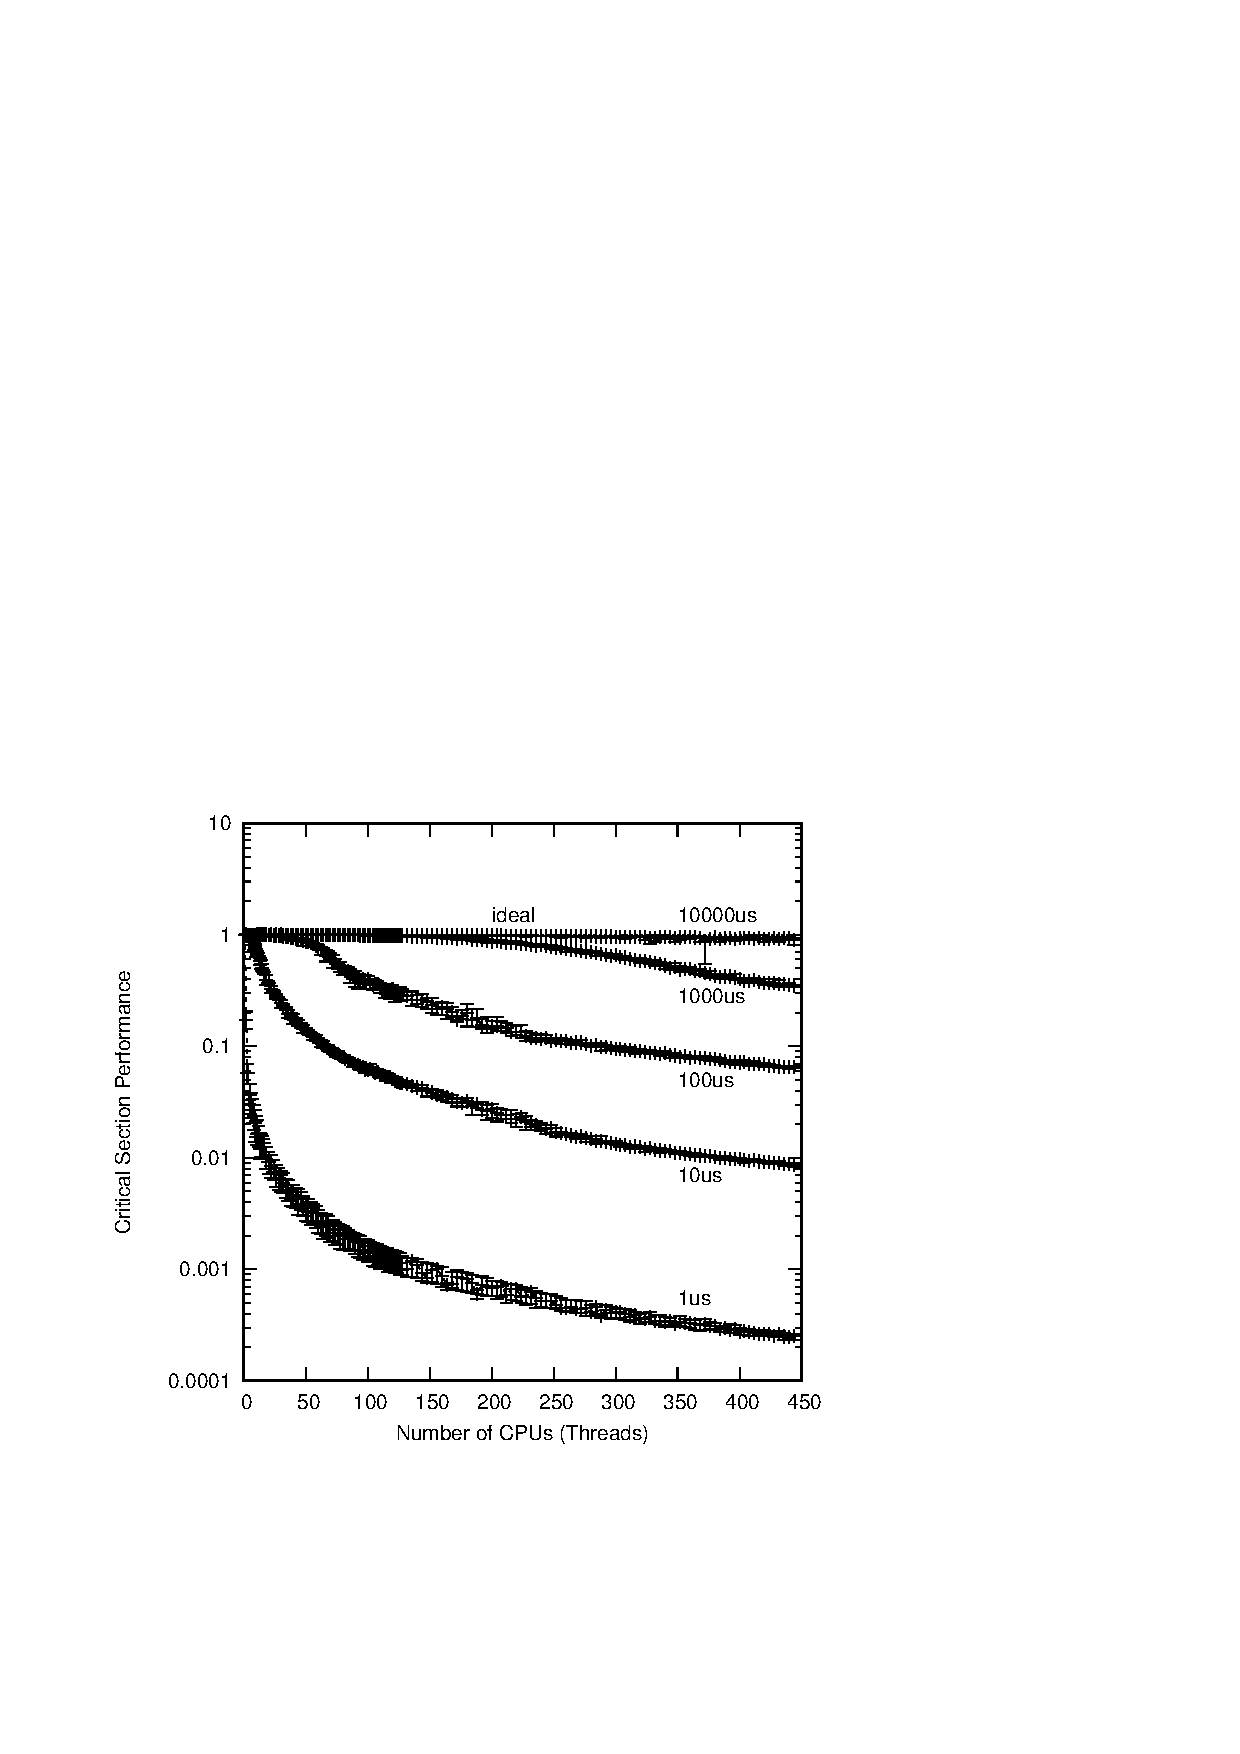
\includegraphics{CodeSamples/toolsoftrade/rwlockscale}}
\caption{Reader-Writer Lock Scalability}
\label{fig:toolsoftrade:Reader-Writer Lock Scalability}
\end{figure}

Figure~\ref{fig:toolsoftrade:Reader-Writer Lock Scalability} 에서는 테스트를
코어당 2개 하드웨어 쓰레드를 지원해 소프트웨어에는 총 128개의 CPU가 존재하는
것으로 보이는 64-코어 \Power{5} 시스템에서 돌린 결과입니다.
\co{thinktime} 패러미터는 모든 테스트에서 0 이었고, \co{holdtime} 은 1000
(그림에서는 ``1K''로 표시되었습니다) 부터 1억 (그림에선 ``100M'' 으로
표시됩니다) 까지 값을 변화시켰습니다.
그림으로 그려진 실제 값은 다음과 같습니다:
\begin{equation}
	\frac{L_N}{N L_1}
\end{equation}
여기서 $N$ 은 쓰레드의 갯수이고, $L_N$ 는 $N$ 쓰레드들의 락 획득 횟수, 그리고
$L_1$ 는 쓰레드 하나만 썼을 때의 락 획득 횟수입니다.
이상적인 하드웨어와 소프트웨어 확장성이 주어졌다면, 이 값은 항상 1.0이 될
것입니다.
\iffalse

Figure~\ref{fig:toolsoftrade:Reader-Writer Lock Scalability}
shows the results of running this test on a 64-core \Power{5} system
with two hardware threads per core for a total of 128 software-visible
CPUs.
The \co{thinktime} parameter was zero for all these tests, and the
\co{holdtime} parameter set to values ranging from one thousand (``1K''
on the graph) to 100 million (``100M'' on the graph).
The actual value plotted is:
\begin{equation}
	\frac{L_N}{N L_1}
\end{equation}
where $N$ is the number of threads,
$L_N$ is the number of lock acquisitions by $N$ threads, and
$L_1$ is the number of lock acquisitions by a single thread.
Given ideal hardware and software scalability, this value will always
be 1.0.
\fi

그림에서 보여지듯이, 리더-라이터 락킹의 확장성은 이상적이진 않고, 특히 작은
크기의 크리티컬 섹션에서 더 그렇습니다.
왜 읽기 권한 락 획득이 그렇게 느린지 알아보려면, 모든 락 획득을 원하는
쓰레드들이 \co{pthread_rwlock_t} 데이터를 수정해야 함을 상기해 보십시오.
따라서, 모든 128개의 수행되는 쓰레드들이 리더-라이터 락으로부터 동시에 읽기
권한 락 획득을 하려 하면, 그 쓰레드들은 \co{pathread_rwlock_t} 를 한번씩 반드시
수정해야만 합니다.
운좋은 쓰레드는 곧바로 그렇게 할 수 있을테지만, 가장 불행한 쓰레드는 다른
127개의 쓰레드들이 수정을 완료할 때까지 기다려야 합니다.
이 상황은 CPU 를 추가할수록 나빠지기만 할 겁니다.
\iffalse

As can be seen in the figure, reader-writer locking scalability is
decidedly non-ideal, especially for smaller sizes of critical
sections.
To see why read-acquisition can be so slow, consider
that all the acquiring threads must update the \co{pthread_rwlock_t}
data structure.
Therefore, if all 128 executing threads attempt to
read-acquire the reader-writer lock concurrently, they must update
this underlying \co{pthread_rwlock_t} one at a time.
One lucky thread might do so almost immediately, but the least-lucky
thread must wait for all the other 127 threads to do their updates.
This situation will only get worse as you add CPUs.
\fi

\QuickQuiz{}
	단일 CPU 성능에 비교하는건 좀 심한 거 아닌가요?
	\iffalse

	Isn't comparing against single-CPU throughput a bit harsh?
	\fi
\QuickQuizAnswer{
	전혀요.
	사실, 이 비교는 지나치게 관대한 편입니다.
	더 균형잡힌 비교를 위해선 락을 전혀 사용하지 않는 단일 CPU 성능과
	비교해야 하겠죠.
	\iffalse

	Not at all.
	In fact, this comparison was, if anything, overly lenient.
	A more balanced comparison would be against single-CPU
	throughput with the locking primitives commented out.
	\fi
} \QuickQuizEnd

\QuickQuiz{}
	하지만 1,000 개의 인스트럭션은 크리티컬 섹션 치고 그렇게 작은 크기는
	아니예요. 수십 개의 인스트럭션 정도만을 가지는 훨씬 작은 크리티컬
	섹션이 필요하면 어떻게 해야하죠?
	\iffalse

	But 1,000 instructions is not a particularly small size for
	a critical section.
	What do I do if I need a much smaller critical section, for
	example, one containing only a few tens of instructions?
	\fi
\QuickQuizAnswer{
	읽혀지는 데이터가 \emph{절대} 변하지 않는다면, 거기 접근하는데 어떤
	락도 잡을 필요가 없습니다.
	만약 데이터가 충분히 가끔만 변경된다면, 실행된 단계를 기록해두고, 모든
	쓰레드를 종료시키고, 데이터를 변경한 후, 기록된 단계부터 쓰레드들을
	다시 실행시키면 됩니다.

	다른 방법은 쓰레드당 하나씩의 배타적 락을 두고, 자신의 락을
	획득함으로써 커다란 리더-라이터 락의 읽기 락 획득을 하고, 모든 쓰레드의
	락을 획득함으로써 쓰기 락 획득을 하는 것~\cite{WilsonCHsieh92a}과 같은
	효과를 얻는 것입니다.
	이 방법은 리더들을 위해선 상당히 잘 동작합니다만, 라이터들은 쓰레드의
	수가 늘어날수록 큰 오버헤드를 갖게 만들 수 있습니다.

	그 외의 매우 작은 크리티컬 섹션을 처리하기 위한 방법들은
	Chapter~\ref{chp:Deferred Processing} 에서 다루고 있습니다.
	\iffalse

	If the data being read \emph{never} changes, then you do not
	need to hold any locks while accessing it.
	If the data changes sufficiently infrequently, you might be
	able to checkpoint execution, terminate all threads, change
	the data, then restart at the checkpoint.

	Another approach is to keep a single exclusive lock per
	thread, so that a thread read-acquires the larger aggregate
	reader-writer lock by acquiring its own lock, and write-acquires
	by acquiring all the per-thread locks~\cite{WilsonCHsieh92a}.
	This can work quite well for readers, but causes writers
	to incur increasingly large overheads as the number of threads
	increases.

	Some other ways of handling very small critical sections are
	described in Chapter~\ref{chp:Deferred Processing}.
	\fi
} \QuickQuizEnd

\QuickQuiz{}
	Figure~\ref{fig:toolsoftrade:Reader-Writer Lock Scalability} 에서 100M
	에서의 경우 이외의 값들은 이상적인 선에서 부드럽게 멀어집니다.
	반면, 100M 에서의 값은 64 CPU 에서 갑자기 이상적인 선으로부터
	멀어지는군요.
	또, 100M 값과 10M 값 사이의 거리는 10M 값과 1M 값 사이의 거리보다
	작아요.
	왜 100M 값은 이렇게 남들과 다른거죠?
	\iffalse

	In
	Figure~\ref{fig:toolsoftrade:Reader-Writer Lock Scalability},
	all of the traces other than the 100M trace deviate gently
	from the ideal line.
	In contrast, the 100M trace breaks sharply from the ideal
	line at 64 CPUs.
	In addition, the spacing between the 100M trace and the 10M
	trace is much smaller than that between the 10M trace and the
	1M trace.
	Why does the 100M trace behave so much differently than the
	other traces?
	\fi
\QuickQuizAnswer{
	첫번째 단서는 64 CPU 는 정확히 기계의 128 CPU 의 절반이란 겁니다.
	그 차이는 하드웨어 쓰레딩의 영향입니다.
	이 시스템은 코어당 2개 하드웨어 쓰레드를 가지며 총 64 코어를 갖습니다.
	64 쓰레드보다 적은 쓰레드가 돌 때 까지는 각 쓰레드가 자신의 코어를
	하나씩 갖고 동작합니다.
	하지만 쓰레드의 수가 64를 넘는 순간, 일부 쓰레드들은 코어를 공유해야만
	합니다.
	한 코어를 공유하는 쓰레드들은 일부 하드웨어 자원을 공유해야 하기
	때문에, 한개 코어를 공유하는 두 쓰레드의 성능은 각자 코어 하나씩 가지고
	도는 두 쓰레드의 것에 비해 낮을 수밖에 없습니다.
	따라서 100M 경우의 성능은 리더-라이터 락에 의해 제한되는게 아니라 싱글
	코어에서의 하드웨어 쓰레드간의 하드웨어 자원 공유에 의해 제한되는
	것입니다.

	이건 10M 경우에도 볼 수 있는데, 64 쓰레드까지 일관되게 떨어지던 성능은
	이후 급격하게 떨어져서 100M 경우와 비슷하죠.
	64 쓰레드까지는 10M 경우도 리더-라이터 락의 확장성에 의해 성능이
	제한되지만, 그 이후부터는 싱글 코어에서의 하드웨어 쓰레드간의 하드웨어
	자원 공유로 인해 제한되는 것입니다.
	\iffalse

	Your first clue is that 64 CPUs is exactly half of the 128
	CPUs on the machine.
	The difference is an artifact of hardware threading.
	This system has 64 cores with two hardware threads per core.
	As long as fewer than 64 threads are running, each can run
	in its own core.
	But as soon as there are more than 64 threads, some of the threads
	must share cores.
	Because the pair of threads in any given core share some hardware
	resources, the throughput of two threads sharing a core is not
	quite as high as that of two threads each in their own core.
	So the performance of the 100M trace is limited not by the
	reader-writer lock, but rather by the sharing of hardware resources
	between hardware threads in a single core.

	This can also be seen in the 10M trace, which deviates gently from
	the ideal line up to 64 threads, then breaks sharply down, parallel
	to the 100M trace.
	Up to 64 threads, the 10M trace is limited primarily by reader-writer
	lock scalability, and beyond that, also by sharing of hardware
	resources between hardware threads in a single core.
	\fi
} \QuickQuizEnd

\QuickQuiz{}
	\Power{5} 는 나온지 몇년이 넘었고, 최신 하드웨어는 분명 더 빠를 거예요.
	그런데 왜 리더-라이터 락의 느린 속도에 걱정해야 하죠?
	\iffalse

	\Power{5} is more than a decade old, and new hardware should
	be faster.
	So why should anyone worry about reader-writer locks being slow?
	\fi
\QuickQuizAnswer{
	일반적으로, 최신 하드웨어에선 개선되어 있습니다.
	하지만, 128 CPU 에서 리더-라이터 락이 이상적인 성능을 달성하기 위해선
	100배 이상의 개선이 필요합니다.
	게다가, CPU 의 갯수가 커질수록, 필요한 성능 향상 정도도 커집니다.
	따라서 리더-라이터 락의 성능 문제는 당분간은 존재할 것입니다.
	\iffalse

	In general, newer hardware is improving.
	However, it will need to improve more than two orders of magnitude
	to permit reader-writer lock to achieve ideal performance on
	128 CPUs.
	Worse yet, the greater the number of CPUs, the larger the
	required performance improvement.
	The performance problems of reader-writer locking are therefore
	very likely to be with us for quite some time to come.
	\fi
} \QuickQuizEnd

이런 한계점에도 불구하고, 리더-라이터 락킹은 많은 경우, 예를 들어 리더들이
대기시간이 긴 파일이나 네트워크 I/O 를 해야만 경우 등에 매우 유용합니다.
다른 대안들도 있는데, 그런 것들 중 일부는 Chapter~\ref{chp:Counting} 와
Chapter~\ref{chp:Deferred Processing} 에서 다루겠습니다.
\iffalse

Despite these limitations, reader-writer locking is quite useful in many
cases, for example when the readers must do high-latency file or network I/O.
There are alternatives, some of which will be presented in
Chapters~\ref{chp:Counting} and \ref{chp:Deferred Processing}.
\fi

\subsection{Atomic Operations (\GCC\ Classic)}
\label{sec:toolsoftrade:Atomic Operations (gcc Classic)}

Figure~\ref{fig:toolsoftrade:Reader-Writer Lock Scalability} 가 리더-라이터
락킹의 오버헤드는 크리티컬 섹션이 작을수록 커진다는 것을 보여줬으니, 매우 작은
크리티컬 섹션을 보호할 다른 나은 방안을 찾아봐야 하겠습니다.
그런 한가지 방안은 어토믹 오퍼레이션의 사용입니다.
우린 Listing~\ref{lst:toolsoftrade:Measuring Reader-Writer Lock Scalability} 의
라인~18 에서 \co{__sync_fetch_and_add()} 를 통해 어토믹 오퍼레이션 중 하나를 본
바 있습니다.
이 기능은 첫번째 인자로 참조된 값에 두번째 인자로 주어진 값을 어토믹하게
더하고, 예전 값(이 경우엔 그냥 무시되었었죠)을 리턴합니다.
두개의 쓰레드가 같은 변수에 대해 동시에 \co{__sync_fetch_and_add()} 를 실행하면
변수의 값은 두 더하기 연산이 모두 수행된 값이 됩니다.
\iffalse

Given that
Figure~\ref{fig:toolsoftrade:Reader-Writer Lock Scalability}
shows that the overhead of reader-writer locking is most severe for the
smallest critical sections, it would be nice to have some other way
to protect the tiniest of critical sections.
One such way are atomic operations.
We have seen one atomic operations already, in the form of the
\co{__sync_fetch_and_add()} primitive on line~18 of
Listing~\ref{lst:toolsoftrade:Measuring Reader-Writer Lock Scalability}.
This primitive atomically adds the value of its second argument to
the value referenced by its first argument, returning the old value
(which was ignored in this case).
If a pair of threads concurrently execute \co{__sync_fetch_and_add()} on
the same variable, the resulting value of the variable will include
the result of both additions.
\fi

\GNUC\ 컴파일러는 이외에도 아래와 같이 추가적인 어토믹 오퍼레이션들을
제공하는데,
\co{__sync_fetch_and_sub()},
\co{__sync_fetch_and_or()},
\co{__sync_fetch_and_and()},
\co{__sync_fetch_and_xor()}, 그리고
\co{__sync_fetch_and_nand()} 는 기존 값을 리턴합니다.
기존 값이 아니라 새롭게 바뀐 값이 필요하다면,
\co{__sync_add_and_fetch()},
\co{__sync_sub_and_fetch()},
\co{__sync_or_and_fetch()},
\co{__sync_and_and_fetch()},
\co{__sync_xor_and_fetch()}, 그리고
\co{__sync_nand_and_fetch()} 를 사용할 수 있습니다.
\iffalse

The \GNUC\ compiler offers a number of additional atomic operations,
including \co{__sync_fetch_and_sub()},
\co{__sync_fetch_and_or()},
\co{__sync_fetch_and_and()},
\co{__sync_fetch_and_xor()}, and
\co{__sync_fetch_and_nand()}, all of which return the old value.
If you instead need the new value, you can instead use the
\co{__sync_add_and_fetch()},
\co{__sync_sub_and_fetch()},
\co{__sync_or_and_fetch()},
\co{__sync_and_and_fetch()},
\co{__sync_xor_and_fetch()}, and
\co{__sync_nand_and_fetch()} primitives.
\fi

\QuickQuiz{}
	정말로 이것들이 다 필요한 거 맞나요?
	\iffalse

	Is it really necessary to have both sets of primitives?
	\fi
\QuickQuizAnswer{
	엄격하게 말하면, 아닙니다.
	필요하면 첫번째 분류의 것들을 이용해서 두번째 분류의 것들을 구현할 수가
	있습니다.
	예를 들어, \co{__sync_fetch_and_nand()} 를 이용해서
	아래와 같이 \co{__sync_nand_and_fetch()} 를 구현할 수 있겠죠.
	\iffalse

	Strictly speaking, no.
	One could implement any member of the second set using the
	corresponding member of the first set.
	For example, one could implement \co{__sync_nand_and_fetch()}
	in terms of \co{__sync_fetch_and_nand()} as follows:
	\fi

\vspace{5pt}
\begin{minipage}[t]{\columnwidth}
\scriptsize
\begin{verbatim}
tmp = v;
ret = __sync_fetch_and_nand(p, tmp);
ret = ~ret & tmp;
\end{verbatim}
\end{minipage}
\vspace{5pt}

	비슷하게 \co{__sync_fetch_and_add()}, \co{__sync_fetch_and_sub()},
	그리고 \co{__sync_fetch_and_xor()} 를 그들의 나중값 리턴하는 대응
	함수들을 이용해 구현하는 것도 가능합니다.

	하지만, 이를 대신해주는 기능이 있는 게 프로그래머에게도
	컴파일러/라이브러리를 구현하는 사람에게도 편리할 것입니다.
	\iffalse

	It is similarly possible to implement \co{__sync_fetch_and_add()},
	\co{__sync_fetch_and_sub()}, and \co{__sync_fetch_and_xor()}
	in terms of their post-value counterparts.

	However, the alternative forms can be quite convenient, both
	for the programmer and for the compiler/library implementor.
	\fi
} \QuickQuizEnd

고전적인 compare-and-swap 오퍼레이션은 \co{__sync_bool_compare_and_swap()} 과
\co{__sync_val_compare_and_swap()} 두개의 함수로 제공됩니다.
두 함수 모두 변수의 현재 값이 제시한 값과 같을 경우 어토믹하게 새로운 값으로
변경해 줍니다.
첫번째 함수는 오퍼레이션이 성공하면 1을, 그리고 실패하면 (예를 들어, 기존 값이
제시한 값과 같지 않은 경우) 0을 리턴합니다.
두번째 함수는 기존 값을 리턴합니다. 따라서 리턴받은 값이 제시했던 기존값과
같다면 오퍼레이션이 성공했음을 의미합니다.
앞의 오퍼레이션들이 적용 가능한 영역에선 대부분 compare-and-swap 보다 더
효율적이지만 하나의 변수에 대한 어떤 어토믹 오퍼레이션도 compare-and-swap 을
사용해서 구현 가능하기 때문에, compare-and-swap 오퍼레이션은 ``보편적''이라 할
수 있습니다.
뿐만 아니라 compare-and-swap 오퍼레이션은 더 넓은 어토믹 오퍼레이션 집합의 토대
역할을 할수도 있습니다. 그렇게 만들어진 것들은 보통 복잡도, 확장성, 성능
문제~\cite{MauriceHerlihy90a}를 겪지만요.
\iffalse

The classic compare-and-swap operation is provided by a pair of
primitives, \co{__sync_bool_compare_and_swap()} and
\co{__sync_val_compare_and_swap()}.
Both of these primitive atomically update a location to a new value,
but only if its prior value was equal to the specified old value.
The first variant returns 1 if the operation succeeded and 0 if it
failed, for example, if the prior value was not equal to the specified
old value.
The second variant returns the prior value of the location, which, if
equal to the specified old value, indicates that the operation succeeded.
Either of the compare-and-swap operation is ``universal'' in the sense
that any atomic operation on a single location can be implemented in
terms of compare-and-swap, though the earlier operations are often
more efficient where they apply.
The compare-and-swap operation is also capable of serving as the basis
for a wider set of atomic operations, though the more elaborate of
these often suffer from complexity, scalability, and performance
problems~\cite{MauriceHerlihy90a}.
\fi

\QuickQuiz{}
	이 어토믹 오퍼레이션들이 인스트럭션 집합에서 곧바로 지원하는
	인스트럭션들을 만들어낼 수 있다면, 그게 바로 동작하는 가장 빠른 방법
	아닐까요?
	\iffalse

	Given that these atomic operations will often be able to
	generate single atomic instructions that are directly
	supported by the underlying instruction set, shouldn't
	they be the fastest possible way to get things done?
	\fi
\QuickQuizAnswer{
	불행히도, 아닙니다.
	극명한 반례를 위해 Chapter~\ref{chp:Counting} 을 참고하시기 바랍니다.
	\iffalse

	Unfortunately, no.
	See Chapter~\ref{chp:Counting} for some stark counterexamples.
	\fi
} \QuickQuizEnd

\co{__sync_synchronize()} 함수는
Chapter~\ref{chp:Advanced Synchronization: Memory Ordering} 에서 이야기
되는대로, 컴파일러와 CPU 의 오퍼레이션 재배치 기능을 제한하는 ``메모리 배리어''
를 발생시킵니다.
어떤 경우에는 CPU 의 재배치 가능성은 두고 컴파일러의 오퍼레이션 재배치를
제한하는 것만으로도 충분한데, 이 경우에는
Listing~\ref{lst:toolsoftrade:Measuring Reader-Writer Lock Scalability} 의
라인~28 에서처럼 \co{barrier()} 기능이 사용될 수 있을 겁니다.
어떤 경우에는 컴파일러가 주어진 메모리 접근의 최적화를 하는 것을 막는
것만으로도 충분한 경우가 있을 수 있는데, 이 경우에는 
Listing~\ref{lst:toolsoftrade:Demonstration of Exclusive Locks} 의 라인~17
에서처럼 \co{READ_ONCE()} 함수가 사용될 수 있을 겁니다.
비슷하게, 컴파일러가 특정 메모리로의 쓰기를 최적화해 버리는 것을 막기 위해
\co{WRITE_ONCE()} 기능이 사용될 수 있습니다.
이 마지막 두개의 함수들은 \GCC 에 의해 제공되지는 않습니다만,
Listing~\ref{lst:toolsoftrade:Compiler Barrier Primitive (for GCC)}
에 보인 것처럼 단순하게 구현될 수도 있을 겁니다.
\iffalse

The \co{__sync_synchronize()} primitive issues a ``memory barrier'',
which constrains both the compiler's and the CPU's ability to reorder
operations, as discussed in
Chapter~\ref{chp:Advanced Synchronization: Memory Ordering}.
In some cases, it is sufficient to constrain the compiler's ability
to reorder operations, while allowing the CPU free rein, in which
case the \co{barrier()} primitive may be used, as it in fact was
on line~28 of
Listing~\ref{lst:toolsoftrade:Measuring Reader-Writer Lock Scalability}.
In some cases, it is only necessary to ensure that the compiler
avoids optimizing away a given memory read, in which case the
\co{READ_ONCE()} primitive may be used, as it was on line~17 of
Listing~\ref{lst:toolsoftrade:Demonstration of Exclusive Locks}.
Similarly, the \co{WRITE_ONCE()} primitive may be used to prevent the
compiler from optimizing away a given memory write.
These last three primitives are not provided directly by \GCC,
but may be implemented straightforwardly as shown in
Listing~\ref{lst:toolsoftrade:Compiler Barrier Primitive (for GCC)}.
\fi

\begin{listing}[tb]
{ \scriptsize
\begin{verbbox}
#define ACCESS_ONCE(x) (*(volatile typeof(x) *)&(x))
#define READ_ONCE(x) \
            ({ typeof(x) ___x = ACCESS_ONCE(x); ___x; })
#define WRITE_ONCE(x, val) ({ ACCESS_ONCE(x) = (val); })
#define barrier() __asm__ __volatile__("": : :"memory")
\end{verbbox}
}
\centering
\theverbbox
\caption{Compiler Barrier Primitive (for \GCC)}
\label{lst:toolsoftrade:Compiler Barrier Primitive (for GCC)}
\end{listing}

\QuickQuiz{}
	\co{ACCESS_ONCE()} 에 무슨 일이 벌어진거죠?
	\iffalse

	What happened to \co{ACCESS_ONCE()}?
	\fi
\QuickQuizAnswer{
	2018년 초 기준으로, 리눅스 커널의 \co{ACCESS_ONCE()} 는 읽기와 쓰기를
	위한 목적으로 각각 \co{READ_ONCE()} 와 \co{WRITE_ONCE()} 로
	교체되었습니다~\cite{JonCorbet2012ACCESS:ONCE,
	JonathanCorbet2014ACCESS:ONCEcompilerBugs,
	MarkRutland2017ACCESS:ONCE:remove}.
	\co{ACCESS_ONCE()} 는 RCU 코드에 도움을 주는 역할로 소개되었지만,
	그후에 core API 로 격상되었습니다~\cite{
	PaulEMcKenney2007ACCESS:ONCE:rcu,
	LinusTorvalds2008ACCESS:ONCE:move}.
	리눅스 커널의 \co{READ_ONCE()} 와 \co{WRITE_ONCE()} 는 커다란 구조체에
	access-once 의미를 제공하면서도 이 구조체가 하나의 기계 인스트럭션으로
	로드되고 스토어 될 수 없을 경우에는 load-store tearing 이 일어날 수
	있게 하기 위해 원래의 \co{ACCESS_ONCE()} 와는 상당히 다르게 보이는
	복잡한 형태로 진화했습니다.
	\iffalse

	As of early 2018, the Linux kernel's \co{ACCESS_ONCE()} is being
	replaced by \co{READ_ONCE()} and \co{WRITE_ONCE()} for reads and
	writes, respectively~\cite{JonCorbet2012ACCESS:ONCE,
	JonathanCorbet2014ACCESS:ONCEcompilerBugs,
	MarkRutland2017ACCESS:ONCE:remove}.
	\co{ACCESS_ONCE()} was introduced as a helper in RCU code, but was
	promoted to core API soon afterward~\cite{
	PaulEMcKenney2007ACCESS:ONCE:rcu,
	LinusTorvalds2008ACCESS:ONCE:move}.
	Linux kernel's \co{READ_ONCE()} and \co{WRITE_ONCE()} have
	evolved into complex forms that look quite different than
	the original \co{ACCESS_ONCE()} implementation due to the
	need to support access-once semantics for large structures,
	but with the possibility of load/store tearing if the structure
	cannot be loaded and stored with a single machine instruction.
	\fi
} \QuickQuizEnd

\subsection{Atomic Operations (C11)}
\label{sec:toolsoftrade:Atomic Operations (C11)}

C11 표준은 어토믹 오퍼레이션들을 추가했는데, 이는 로드 (\co{atomic_load()}),
스토어 (\co{atomic_store()}), 메모리 배리어 (\co{atomic_thread_fence()} 와
\co{atomic_signal_fence()}), 그리고 read-modify-write 어토믹 오퍼레이션들을
포함합니다.
Read-modify-write 어토믹 오퍼레이션들은
\co{atomic_fetch_add()},
\co{atomic_fetch_sub()},
\co{atomic_fetch_and()},
\co{atomic_fetch_xor()},
\co{atomic_exchange()},
\co{atomic_compare_exchange_strong()},
그리고
\co{atomic_compare_exchange_weak()} 를 포함합니다.
이것들은
Section~\ref{sec:toolsoftrade:Atomic Operations (gcc Classic)} 에서 설명한
것들과 비슷한 방식으로 동작합니다만 모든 오퍼레이션의 \co{_explicit} 변종들은
메모리 순서 인자를 추가로 받습니다.
메모리 순서 인자 없이는, 모든 어토믹 오퍼레이션들은 완전히 순서를맞추고, 인자가
주어진다면 완화된 순서규칙을 허용합니다.
예를 들어, ``\co{atomic_load_explicit(&a, memory_order_relaxed)}'' 는 리눅스
커널의 ``\co{READ_ONCE()}'' 와 대략적으로 유사합니다.\footnote{
	메모리 순서 규칙은
	Chapter~\ref{chp:Advanced Synchronization: Memory Ordering} 와
	Appendix~\ref{chp:app:whymb:Why Memory Barriers?}
	에서 더 자세히 설명됩니다.}
\iffalse

The C11 standard added atomic operations,
including loads (\co{atomic_load()}),
stores (\co{atomic_store()}),
memory barriers (\co{atomic_thread_fence()} and
\co{atomic_signal_fence()}), and read-modify-write atomics.
The read-modify-write atomics include
\co{atomic_fetch_add()},
\co{atomic_fetch_sub()},
\co{atomic_fetch_and()},
\co{atomic_fetch_xor()},
\co{atomic_exchange()},
\co{atomic_compare_exchange_strong()},
and
\co{atomic_compare_exchange_weak()}.
These operate in a manner similar to those described in
Section~\ref{sec:toolsoftrade:Atomic Operations (gcc Classic)},
but with the addition of memory-order arguments to \co{_explicit}
variants of all of the operations.
Without memory-order arguments, all the atomic operations are
fully ordered, and the arguments permit weaker orderings.
For example, ``\co{atomic_load_explicit(&a, memory_order_relaxed)}''
is vaguely similar to the Linux kernel's ``\co{READ_ONCE()}''.\footnote{
	Memory ordering is described in more detail in
	Chapter~\ref{chp:Advanced Synchronization: Memory Ordering} and
	Appendix~\ref{chp:app:whymb:Why Memory Barriers?}.}
\fi

C11 어토믹 오퍼레이션들의 한가지 한계점은 특수한 어토믹 타입들에만 적용된다는
것으로, 문제가 될 수 있습니다.
따라서 \GNUC\ 컴파일러는
\co{__atomic_load()},
\co{__atomic_load_n()},
\co{__atomic_store()},
\co{__atomic_store_n()} 등을 제공합니다.
이런 기능들은 C11 에서 대응되는 것들과 동일한 semantic 을 제공합니다만, atomic
타입이 아닌 평범한 객체에 대해서도 사용될 수도 있습니다.
이 기능들 중 일부는 이 목록의 메모리 순서 인자를 받을 수도 있습니다:
\iffalse

One restriction of the C11 atomics is that they apply only to special
atomic types, which can be problematic.
The \GNUC\ compiler therefore provides atomic intrinsics, including
\co{__atomic_load()},
\co{__atomic_load_n()},
\co{__atomic_store()},
\co{__atomic_store_n()}
\co{__atomic_thread_fence()}, etc.
These intrinsics offer the same semantics as their C11 counterparts,
but may be used on plain non-atomic objects.
Some of these intrinsics may be passed a memory-order argument from
this list:
\fi
\co{__ATOMIC_RELAXED},
\co{__ATOMIC_CONSUME},
\co{__ATOMIC_ACQUIRE},
\co{__ATOMIC_RELEASE},
\co{__ATOMIC_ACQ_REL}, and
\co{__ATOMIC_SEQ_CST}.

\subsection{Per-Thread Variables}
\label{sec:toolsoftrade:Per-Thread Variables}

Thread-specific 데이터, thread-local storage, 그리고 그 외의 다른 이름으로도
불리는 per-thread 변수는 Chapter~\ref{chp:Counting} 와~\ref{chp:Data Ownership}
에서 알아보겠지만, 동시성 코드에서 매우 많이 사용됩니다.
POSIX 는 하나의 per-thread 변수를 만들기 위해 (그리고 연관된 키를 리턴받기
위해) \co{pthrad_key_create()} 함수를, 해당 키에 연관된 해당 per-thread 변수를
삭제하기 위해 \co{pthread_key_delete()} 를, 현재 쓰레드의 특정 키에 연관된
변수에 값을 지정하기 위해 \co{pthread_setspecific()} 을, 그리고 그 값을 받기
위해 \co{pthread_getspecific()} 을 제공합니다.
\iffalse

Per-thread variables, also called thread-specific data, thread-local
storage, and other less-polite names, are used extremely
heavily in concurrent code, as will be explored in
Chapters~\ref{chp:Counting} and~\ref{chp:Data Ownership}.
POSIX supplies the \co{pthread_key_create()} function to create a
per-thread variable (and return the corresponding key),
\co{pthread_key_delete()} to delete the per-thread variable corresponding
to key,
\co{pthread_setspecific()} to set the value of the current thread's
variable corresponding to the specified key,
and \co{pthread_getspecific()} to return that value.
\fi

여러개의 (\GCC 를 포함한) 컴파일러들이 변수를 per-thread 로 지정하기 위해
변수의 정의에 사용될 수 있는 \co{__thread} 지시어를 제공합니다.
그렇게 지정되면 해당 변수의 이름은 현재 쓰레드의 해당 변수의 인스턴스에
접근하기 위해 평범하게 사용될 수 있습니다.
물론, \co{__thread} 는 POSIX thread-specific data 보다 사용하기가 쉽고,
\co{__thread} 는 \GCC 나 \co{__thread} 를 지원하는 컴파일러에서만 빌드될
코드에서는 일반적으로 더 선호됩니다.

다행히도, C11 표준은 \co{__thread} 대신 사용될 수 있는 \co{Thread_local}
키워드를 새로 도입했습니다.
시간이 충분히 지나면, 이 새로운 키워드는 \co{__thread} 의 간편한 사용성과 POSIX
thread-specific data 의 호환성을 결합해낼 겁니다.
\iffalse

A number of compilers (including \GCC) provide a \co{__thread} specifier
that may be used in a variable definition to designate that variable
as being per-thread.
The name of the variable may then be used normally to access the
value of the current thread's instance of that variable.
Of course, \co{__thread} is much easier to use than the POSIX
thead-specific data, and so \co{__thread} is usually preferred for
code that is to be built only with \GCC\ or other compilers supporting
\co{__thread}.

Fortunately, the C11 standard introduced a \co{_Thread_local} keyword
that can be used in place of \co{__thread}.
In the fullness of time, this new keyword should combine the ease of use
of \co{__thread} with the portability of POSIX thread-specific data.
\fi

\section{Alternatives to POSIX Operations}
\label{sec:toolsoftrade:Alternatives to POSIX Operations}

불행히도, 쓰레딩 오퍼레이션들, 락킹 기능들, 그리고 어토믹 오퍼레이션들은 다양한
표준 위원회가 그것들을 표준화 하기 전부터 매우 많이 사용되었습니다.
그 결과, 이 오퍼레이션들이 지원되는 방법에 상당한 다양성이 있습니다.
역사적 이유로든 특정 환경에서 더 나은 성능을 얻기 위해서든, 어셈블리 언어로
구현된 오퍼레이션들도 여전히 많습니다.
예를 들어, \GCC 의 \co{__sync_} 류 기능들은 완전한 메모리 순서 의미를 제공해서
많은 개발자들이 메모리 순서 의미가 요구되지 않는 상황을 위한 각자의 구현을
만들도록 이끈 바 있습니다.
다음 섹션들은 리눅스 커널에서의 일부 대안들과 이 책의 예제 코드에서 사용된
역사적 기능들 일부를 보입니다.
\iffalse

Unfortunately, threading operations, locking primitives, and atomic
operations were in reasonably wide use long before the various standards
committees got around to them.
As a result, there is considerable variation in how these operations
are supported.
It is still quite common to find these operations implemented in
assembly language, either for historical reasons or to obtain better
performance in specialized circumstances.
For example, \GCC's \co{__sync_} family of primitives all provide full
memory-ordering semantics, which in the past motivated many developers
to create their own implementations for situations where the full memory
ordering semantics are not required.
The following sections show some alternatives from the Linux kernel
and some historical primitives used by this book's sample code.
\fi

\subsection{Organization and Initialization}
\label{sec:toolsoftrade:Organization and Initialization}

많은 환경들이 특수한 초기화 코드를 필요로 하지 않긴 하지만, 이 책의 샘플 코드는
\co{pthread_t} 로부터 연속적인 정수들 사이의 매핑을 초기화하는 \co{smp_init()}
함수의 호출로 시작합니다.
Userspace RCU 라이브러리는 비슷하게 \co{rcu_init()} 호출을 필요로 합니다.
이런 함수 호출들은 생성자를 지원하는 (\GCC 와 같은) 환경에서는 숨겨질 수 있긴
하지만, userspace RCU 라이브러리에 의해 지원되는 대부분의 RCU 버전들은 각
쓰레드가 쓰레드 생성 직후 \co{rcu_register_thread()} 를, 그리고 쓰레드 종료
전에 \co{rcu_unregister_thread()} 를 호출할 것을 필요로 합니다.

리눅스 커널의 경우, 커널이 특수한 초기화 코드로의 호출을 필요로 하는지 여부나
커널의 부팅 시점 코드가 실제로는 필요시되는 초기화 코드인가 여부와 같은 것들은
철학적인 질문입니다.
\iffalse

Although many environments do not require any special initialization
code, the code samples in this book start with a call to \co{smp_init()},
which initializes a mapping from \co{pthread_t} to consecutive integers.
The userspace RCU library similarly requires a call to \co{rcu_init()}.
Although these calls can be hidden in environments (such as that of
\GCC) that support constructors,
most of the RCU flavors supported by the userspace RCU library
also require each thread invoke \co{rcu_register_thread()} upon thread
creation and \co{rcu_unregister_thread()} before thread exit.

In the case of the Linux kernel, it is a philosophical question as to
whether the kernel does not require calls to special initialization
code or whether the kernel's boot-time code is in fact the required
initialization code.
\fi

\subsection{Thread Creation, Destruction, and Control}
\label{sec:toolsoftrade:Thread Creation, Destruction, and Control}

리눅스 커널은 kthread 들의 정보를 관리하는데에 \co{struct task_struct}
포인터를, 그것들을 생성하는데 \co{kthread_create()} 를, 그것들이 멈출 것을
외부로 제안하는데에 (POSIX 에는 똑같은 일을 하는 게 없습니다)
\co{kthread_should_stop()} 을, 그것들이 멈추길 기다리는데에 \co{kthread_stop()}
을, 그리고 지정된 시간동안의 대기를 위해서
\co{schedule_timeout_interruptible()} 을 사용합니다.
몇가지 더 kthread 관리 API 들이 있습니다만, 이것만으로도 괜찮은 시작점과 검색어
키워드가 됩니다.

CodeSamples API 는 ``thread'' 에 집중하는데, 이는 제어를 위한 하나의
위치입니다.\footnote{
	비슷한 소프트웨어 구성물을 위한 많은 다른 이름들이 있는데, ``process'',
	``task'', ``fiber'', ``event'', 등등이 있습니다.
	이것들 모두에 비슷한 설계 철학이 적용됩니다.}
그런 쓰레드 각각은 \co{thread_id_t} 타입의 식별자를 가지고, 동시에 수행중인
어떤 두 쓰레드도 같은 식별자를 갖지는 않습니다.
쓰레드들은 program counter 와 stack 을 포함하는 쓰레드별 지역적 상태\footnote{
	순환정의에서는 이게 어떻게 될까요?}
를 제외하고는 어떤 것도 공유하지 않습니다.

이 쓰레드 API 는
Listing~\ref{lst:toolsoftrade:Thread API} 에 보여져 있으며, 이것들 각각은 뒤의
섹션들에서 설명됩니다.
\iffalse

The Linux kernel uses
\co{struct task_struct} pointers to track kthreads,
\co{kthread_create()} to create them,
\co{kthread_should_stop()} to externally suggest that they stop
(which has no POSIX equivalent),
\co{kthread_stop()} to wait for them to stop, and
\co{schedule_timeout_interruptible()} for a timed wait.
There are quite a few additional kthread-management APIs, but this
provides a good start, as well as good search terms.

The CodeSamples API focuses on ``threads'', which are a locus of
control.\footnote{
	There are many other names for similar software constructs, including
	``process'', ``task'', ``fiber'', ``event'', and so on.
	Similar design principles apply to all of them.}
Each such thread has an identifier of type \co{thread_id_t},
and no two threads running at a given time will have the same
identifier.
Threads share everything except for per-thread local state,\footnote{
	How is that for a circular definition?}
which includes program counter and stack.

The thread API is shown in
Listing~\ref{lst:toolsoftrade:Thread API}, and members are described in the
following sections.
\fi

\begin{listing*}[tbp]
{ \scriptsize
\begin{verbbox}
int smp_thread_id(void)
thread_id_t create_thread(void *(*func)(void *), void *arg)
for_each_thread(t)
for_each_running_thread(t)
void *wait_thread(thread_id_t tid)
void wait_all_threads(void)
\end{verbbox}
}
\centering
\theverbbox
\caption{Thread API}
\label{lst:toolsoftrade:Thread API}
\end{listing*}

\subsubsection{\tco{create_thread()}}

\co{create_thread()} 기능은 새로운 쓰레드를 생성하고, \co{create_thread()} 의
첫번째 인자로 명시된 \co{func} 함수에서부터 이 새로운 쓰레드의 수행을
시작하는데, 이때 \co{create_thread()} 의 두번째 인자로 명시된 인자를
넘겨줍니다.
이렇게 새로 생성된 쓰레드는 \co{func} 로 명시된 함수가 리턴할 때에 종료됩니다.
\co{create_thread()} 기능은 새로 생성된 자식 쓰레드에 연관된 \co{thread_id_t}
를 리턴합니다.

이 기능은 프로그램의 수행동안 생성된 쓰레드의 갯수를 내부적으로 세다가, 만약
\co{NR_THREADS} 보다 많은 쓰레드가 생성되면 프로그램을 종료시킵니다.
\co{NR_THREADS} 는 컴파일 시점에서 지정되는 상수로, 그 값은 수정될 수도 있지만
일부 시스템에서는 허용 가능한 쓰레드의 수에 최대값이 정해져 있을 수 있습니다.
\iffalse

The \co{create_thread()} primitive creates a new thread,
starting the new thread's execution
at the function \co{func} specified by \co{create_thread()}'s
first argument, and passing it the argument specified by
\co{create_thread()}'s second argument.
This newly created thread will terminate when it returns from the
starting function specified by \co{func}.
The \co{create_thread()} primitive returns the \co{thread_id_t}
corresponding to the newly created child thread.

This primitive will abort the program if more than \co{NR_THREADS}
threads are created, counting the one implicitly created by running
the program.
\co{NR_THREADS} is a compile-time constant that may be modified,
though some systems may have an upper bound for the allowable number
of threads.
\fi

\subsubsection{\tco{smp_thread_id()}}

\co{create_thread()} 로부터 리턴받는 \co{thread_id_t} 는 시스템에 종속적이므로,
\co{smp_thread_id()} 기능은 요청받은 쓰레드에 연관된 쓰레드 인덱스를
리턴합니다.
이 인덱스는 프로그램이 시작한 이래로 존재한 쓰레드의 최대 숫자보다 작을 것이
보장되어지고, 따라서 bitmask, 배열 인덱스, 등등에 유용합니다.
\iffalse

Because the \co{thread_id_t} returned from \co{create_thread()} is
system-dependent, the \co{smp_thread_id()} primitive returns a thread
index corresponding to the thread making the request.
This index is guaranteed to be less than the maximum number of threads
that have been in existence since the program started,
and is therefore useful for bitmasks, array indices, and
the like.
\fi

\subsubsection{\tco{for_each_thread()}}

\co{for_each_thread()} 매크로는 생성되면 \emph{존재하게 될} 모든 쓰레드들을
포함해서 모든 존재하는 쓰레드들을 루프합니다.
이 매크로는 Section~\ref{sec:toolsoftrade:Per-Thread Variables} 에서 보게 될
per-thread 변수들을 다루는데에 유용합니다.
\iffalse

The \co{for_each_thread()} macro loops through all threads that exist,
including all threads that \emph{would} exist if created.
This macro is useful for handling per-thread variables as will be
seen in Section~\ref{sec:toolsoftrade:Per-Thread Variables}.
\fi

\subsubsection{\tco{for_each_running_thread()}}

\co{for_each_running_thread()} 매크로는 현재 존재하는 쓰레드들만을 루프합니다.
필요할 경우 쓰레드 생성과 삭제에 동기화를 하는 것은 호출자의 역할입니다.
\iffalse

The \co{for_each_running_thread()}
macro loops through only those threads that currently exist.
It is the caller's responsibility to synchronize with thread
creation and deletion if required.
\fi

\subsubsection{\tco{wait_thread()}}

\co{wait_thread()} 기능은 거기 넘겨주는 \co{thread_id_t} 로 명시되는 쓰레드의
완료를 기다립니다.
이 기능은 명시된 쓰레드의 수행에 어떠한 간섭도 끼치지 않습니다; 그저, 그것을
기다릴 뿐입니다.
\co{wait_thread()} 는 연관된 쓰레드로부터 리턴된 값을 리턴함을 알아두세요.
\iffalse

The \co{wait_thread()} primitive waits for completion of the thread
specified by the \co{thread_id_t} passed to it.
This in no way interferes with the execution of the specified thread;
instead, it merely waits for it.
Note that \co{wait_thread()} returns the value that was returned by
the corresponding thread.
\fi

\subsubsection{\tco{wait_all_threads()}}

\co{wait_all_threads()} 기능은 현재 수행중인 모든 쓰레드의 완료를 기다립니다.
필요하다면 쓰레드 생성, 소멸과 동기화를 맞추는건 호출자의 역할입니다.
하지만, 이 기능은 일반적으로 프로그램 수행 종료 시에 정리를 하는데에
사용되므로, 그런 동기화는 보통은 필요하지 않습니다.
\iffalse

The \co{wait_all_threads()}
primitive waits for completion of all currently running threads.
It is the caller's responsibility to synchronize with thread creation
and deletion if required.
However, this primitive is normally used to clean up at the end of
a run, so such synchronization is normally not needed.
\fi

\subsubsection{Example Usage}

Listing~\ref{lst:toolsoftrade:Example Child Thread}
는 hello-world 같은 자식 쓰레드의 예제를 보입니다.
앞서서 이야기 되었듯, 각각의 쓰레드는 자신의 스택을 할당받고, 따라서 각각의
쓰레드는 자신만의 \co{arg} 인자와 \co{myarg} 변수를 갖습니다.
각각의 자식은 단순히 각자의 인자와 각자의 \co{smp_thread_id()} 를 종료되기 전에
출력합니다.
Line~7 의 \co{return} 문은 쓰레드를 종료시키고, 누구든 이 쓰레드에 대해
\co{wait_thread()} 를 호출한 쪽에 \co{NULL} 을 리턴함을 알아두시기 바랍니다.
\iffalse

Listing~\ref{lst:toolsoftrade:Example Child Thread}
shows an example hello-world-like child thread.
As noted earlier, each thread is allocated its own stack, so
each thread has its own private \co{arg} argument and \co{myarg} variable.
Each child simply prints its argument and its \co{smp_thread_id()}
before exiting.
Note that the \co{return} statement on line~7 terminates the thread,
returning a \co{NULL} to whoever invokes \co{wait_thread()} on this
thread.
\fi

\begin{listing}[tbp]
{ \scriptsize
\begin{verbbox}
  1 void *thread_test(void *arg)
  2 {
  3   int myarg = (int)arg;
  4
  5   printf("child thread %d: smp_thread_id() = %d\n",
  6          myarg, smp_thread_id());
  7   return NULL;
  8 }
\end{verbbox}
}
\centering
\theverbbox
\caption{Example Child Thread}
\label{lst:toolsoftrade:Example Child Thread}
\end{listing}

그 부모 프로그램이
Listing~\ref{lst:toolsoftrade:Example Parent Thread}
에 보여져 있습니다.
이 프로그램은 line~6 에서 쓰레드 시스템을 초기화 하기 위해 \co{smp_init()} 를
호출하고, line~7-14 에서 인자들을 분석한 후, line~15 에서 자신의 존재를
공지합니다.
이 프로그램은 이어서 지정된 수의 자식 쓰레드들을 line~16-17 에서 생성하고,
그것들이 완료되기를 line~18 에서 기다립니다.
\co{wait_all_threads()} 는 여기선 그 값이 \co{NULL} 로써 큰 의미가 없는,
쓰레드들이 리턴하는 값들을 무시함을 알아두시기 바랍니다.
\iffalse

The parent program is shown in
Listing~\ref{lst:toolsoftrade:Example Parent Thread}.
It invokes \co{smp_init()} to initialize the threading system on
line~6,
parses arguments on lines~7-14, and announces its presence on line~15.
It creates the specified number of child threads on lines~16-17,
and waits for them to complete on line~18.
Note that \co{wait_all_threads()} discards the threads return values,
as in this case they are all \co{NULL}, which is not very interesting.
\fi

\begin{listing}[tbp]
{ \scriptsize
\begin{verbbox}
  1 int main(int argc, char *argv[])
  2 {
  3   int i;
  4   int nkids = 1;
  5
  6   smp_init();
  7   if (argc > 1) {
  8     nkids = strtoul(argv[1], NULL, 0);
  9     if (nkids > NR_THREADS) {
 10       fprintf(stderr, "nkids=%d too big, max=%d\n",
 11         nkids, NR_THREADS);
 12       usage(argv[0]);
 13     }
 14   }
 15   printf("Parent spawning %d threads.\n", nkids);
 16   for (i = 0; i < nkids; i++)
 17     create_thread(thread_test, (void *)i);
 18   wait_all_threads();
 19   printf("All threads completed.\n", nkids);
 20   return EXIT_SUCCESS;
 21 }
\end{verbbox}
}
\centering
\theverbbox
\caption{Example Parent Thread}
\label{lst:toolsoftrade:Example Parent Thread}
\end{listing}

\QuickQuiz{}
	리눅스 커널의 \co{fork()} 와 \co{wait()} 대체물은 어디갔죠?
	\iffalse

	What happened to the Linux-kernel equivalents to \co{fork()}
	and \co{wait()}?
	\fi
\QuickQuizAnswer{
	그런건 없습니다.
	리눅스 커널 내에서 실행되는 모든 태스크들은 메모리를 공유합니다. 당신이
	거대한 메모리 매핑을 손으로 일일히 할 생각이 아니라면 말이죠.
	\iffalse

	They don't really exist.
	All tasks executing within the Linux kernel share memory,
	at least unless you want to do a huge amount of memory-mapping
	work by hand.
	\fi
} \QuickQuizEnd

\subsection{Locking}
\label{sec:toolsoftrade:Locking}

리눅스 커널의 락킹 API 가운데 처음 알아보기 시작하는데 좋은 부분집합들이
Listing~\ref{lst:toolsoftrade:Locking API} 에 보여져 있는데, 각각의 API 원소는
다음 섹션들에서 설명됩니다.
이 책의 CodeSamples 락킹 API 는 리눅스 커널의 그것을 거의 유사하게 따라갑니다.
\iffalse

A good starting subset of the Linux kernel's locking API is shown in
Listing~\ref{lst:toolsoftrade:Locking API},
each API element being described in the following sections.
This book's CodeSamples locking API closely follows that of the Linux kernel.
\fi

\begin{listing}[tbp]
{ \scriptsize
\begin{verbbox}
void spin_lock_init(spinlock_t *sp);
void spin_lock(spinlock_t *sp);
int spin_trylock(spinlock_t *sp);
void spin_unlock(spinlock_t *sp);
\end{verbbox}
}
\centering
\theverbbox
\caption{Locking API}
\label{lst:toolsoftrade:Locking API}
\end{listing}

\subsubsection{\tco{spin_lock_init()}}

\co{spin_lock_init()} 기능은 명시된 \co{spinlock_t} 변수를 초기화하며, 이
변수가 다른 spinlock 기능들에 전달되기 전에 반드시 호출되어야 합니다.
\iffalse

The \co{spin_lock_init()} primitive initializes the specified
\co{spinlock_t} variable, and must be invoked before
this variable is passed to any other spinlock primitive.
\fi

\subsubsection{\tco{spin_lock()}}

\co{spin_lock()} 기능은 필요하다면 해당 스핀락이 획득 가능해질 때까지 기다리고
명시된 스핀락을 획득합니다.
Pthread 와 같은 일부 환경에서 이 기다림은 ``spinning'' 을 포함할 수도 있는
반면에, 리눅스 커널과 같은 다른 경우에는 blocking 을 포함합니다.

여기서의 핵심은, 언제든 하나의 스핀락은 하나의 쓰레드만이 잡을 수 있다는
것입니다.
\iffalse

The \co{spin_lock()} primitive acquires the specified spinlock,
if necessary, waiting until the spinlock becomes available.
In some environments, such as pthreads, this waiting will involve
``spinning'', while
in others, such as the Linux kernel, it will involve blocking.

The key point is that only one thread may hold a spinlock at any
given time.
\fi

\subsubsection{\tco{spin_trylock()}}

\co{spin_trylock()} 기능은 곧바로 스핀락을 획득할 수 있을 때에만 명시된
스핀락을 획득합니다.
스핀락을 획득할 수 있었다면 \co{true} 를 리턴하고 그렇지 않다면 \co{false} 를
리턴합니다.
\iffalse

The \co{spin_trylock()} primitive acquires the specified spinlock,
but only if it is immediately available.
It returns \co{true} if it was able to acquire the spinlock and
\co{false} otherwise.
\fi

\subsubsection{\tco{spin_unlock()}}

\co{spin_unlock()} 기능은 명시된 스핀락을 놓아주어서 다른 쓰레드들이 해당
스핀락을 획득할 수 있도록 해줍니다.
\iffalse

The \co{spin_unlock()} primitive releases the specified spinlock,
allowing other threads to acquire it.
\fi

% \emph{@@@ likely need to add reader-writer locking.}

\subsubsection{Example Usage}

변수 \co{counter} 를 보호하는데에 \co{mutex} 라는 이름의 스핀락을 다음과 같이
사용할 수 있습니다:
\iffalse

A spinlock named \co{mutex} may be used to protect a variable
\co{counter} as follows:
\fi

\vspace{5pt}
\begin{minipage}[t]{\columnwidth}
\small
\begin{verbatim}
spin_lock(&mutex);
counter++;
spin_unlock(&mutex);
\end{verbatim}
\end{minipage}
\vspace{5pt}

\QuickQuiz{}
	변수 {\tt counter} 의 값이 {\tt mutex} 의 보호 없이 증가된다면 어떤
	문제가 있을 수 있나요?
	\iffalse

	What problems could occur if the variable {\tt counter} were
	incremented without the protection of {\tt mutex}?
	\fi
\QuickQuizAnswer{
	Load-store 아키텍쳐의 CPU 들에서라면, {\tt counter} 의 값 증가 연산은
	다음과 같은 형태로 컴파일 될 수 있습니다:
	\iffalse

	On CPUs with load-store architectures, incrementing {\tt counter}
	might compile into something like the following:
	\fi

\vspace{5pt}
\begin{minipage}[t]{\columnwidth}
\small
\begin{verbatim}
LOAD counter,r0
INC r0
STORE r0,counter
\end{verbatim}
\end{minipage}
\vspace{5pt}

	그런 기계에서라면, 두개의 쓰레드가 동시에 {\tt counter} 의 값을
	읽어오고, 각자 그 값을 증가시킨 후, 각각 그 결과를 저장할 수 있습니다.
	그렇게 되면 {\tt counter} 의 새로운 값은 두개의 쓰레드가 각각 그 값을
	증가시켰음에도 기존에 비해 1만큼만 클 것입니다.
	\iffalse

	On such machines, two threads might simultaneously load the
	value of {\tt counter}, each increment it, and each store the
	result.
	The new value of {\tt counter} will then only be one greater
	than before, despite two threads each incrementing it.
	\fi
} \QuickQuizEnd

하지만, \co{spin_lock()} 과 \co{spin_unlock()} 기능들은 성능상의 문제가 있는데,
Section~\ref{sec:toolsoftrade:Performance} 에서 다루어집니다.
\iffalse

However, the \co{spin_lock()} and \co{spin_unlock()} primitives
do have performance consequences, as will be seen in
Section~\ref{sec:toolsoftrade:Performance}.
\fi

\subsection{Atomic Operations}
\label{sec:toolsoftrade:Atomic Operations}

리눅스 커널은 다양한 어토믹 오퍼레이션들을 제공합니다만, \co{atomic_t} 타입으로
정의되어있는 것들이 좋은 시작점이 될겁니다.
일반적인 non-tearing read 와 store 들은 \co{atomic_read()} 와 \co{atomic_set()}
으로 각각 제공됩니다.
Acquire load 는 \co{smp_load_acquire()} 로, release store 는
\co{smp_store_release()} 로 제공됩니다.

값을 리턴하지 않는 fetch-and-add 오퍼레이션들은 \co{atomic_add()},
\co{atomic_sub()}, \co{atomic_inc()}, 그리고 \co{atomic_dec()} 으로 제공됩니다.
값이 0이 되는 경우에 대한 알림을 리턴하는 어토믹 값 감소 연산은
\co{atomic_dec_and_test()} 와 \co{atomic_sub_and_test()} 로 제공됩니다.
새로운 값을 리턴하는 어토믹 값 증가 연산은 \co{atomic_add_return()} 으로
제공됩니다.
\co{atomic_add_unless()} 와 \co{atomic_inc_not_zero()} 는 어토믹 변수들의 원래
값이 명시된 값과 다르다면 아무일도 일어나지 않는 조건적 어토믹 오퍼레이션들을
제공합니다 (예컨대, 레퍼런스 카운터를 관리하는데에 이것들이 매우 유용합니다).
\iffalse

The Linux kernel provides a wide variety of atomic operations, but
those defined on type \co{atomic_t} provide a good start.
Normal non-tearing reads and stores are provided by
\co{atomic_read()} and \co{atomic_set()}, respectively.
Acquire load is provided by \co{smp_load_acquire()} and release
store by \co{smp_store_release()}.

Non-value-returning fetch-and-add operations are provided by
\co{atomic_add()}, \co{atomic_sub()}, \co{atomic_inc()}, and
\co{atomic_dec()}, among others.
An atomic decrement that returns a reached-zero indication is provided
by both \co{atomic_dec_and_test()} and \co{atomic_sub_and_test()}.
An atomic add that returns the new value is provided by
\co{atomic_add_return()}.
Both \co{atomic_add_unless()} and \co{atomic_inc_not_zero()} provide
conditional atomic operations, where nothing happens unless the
original value of the atomic variable is different than the value
specified (these are very handy for managing reference counters, for
example).
\fi

어토믹 값 교환 오퍼레이션은 \co{atomic_xchg()} 로 제공되고, 찬양되는
compare-and-swap (CAS) 오퍼레이션은 \co{atomic_cmpxchg()} 로 제공됩니다.
이것들 둘 다 기존 값을 리턴합니다.
리눅스 커널에서는 더 많은 어토믹 RMW 기능들이 사용 가능한데, 리눅스 커널 소스
트리의 \co{Documentation/atomic_ops.txt} 파일을 참고하시기 바랍니다.

이 책의 CodeSamples API 는 리눅스 커널의 것들을 거의 비슷하게 따라합니다.
\iffalse

An atomic exchange operation is provided by \co{atomic_xchg()}, and
the celebrated compare-and-swap (CAS) operation is provided by
\co{atomic_cmpxchg()}.
Both of these return the old value.
Many additional atomic RMW primitives are available in the Linux kernel,
see the \co{Documentation/atomic_ops.txt} file in the Linux-kernel
source tree.

This book's CodeSamples API closely follows that of the Linux kernel.
\fi

\subsection{Per-CPU Variables}
\label{sec:toolsoftrade:Per-CPU Variables}

리눅스 커널은 per-CPU 변수 (CPU 별로 인스턴스를 하나씩 소유하는 변수) 를
정의하기 위해 \co{DEFINE_PER_CPU()} 를, 현재 CPU 가 소유한 특정 per-CPU 변수의
인스턴스를 참조하는데에 \co{this_cpu_ptr()} 를, 특정 CPU 가 소유한 특정 per-CPU
변수의 인스턴스를 접근하는데에 \co{per_cpu()} 를 사용하며, 그 외에도 많은 특수
목적의 per-CPU 오퍼레이션들이 존재합니다.

Listing~\ref{lst:toolsoftrade:Per-Thread-Variable API}
는 이 책의 per-thread-variable API 를 보이는데, 리눅스 커널의 per-CPU-variable
API 의 패턴을 따랐습니다.
이 API 는 쓰레드별 전역변수와 동일한 것을 제공합니다.
엄격하게 말하자면 이 API 가 꼭 필요한 건 아닙니다만\footnote{
	이 API 대신에 \co{__thread} 나 \co{_Thread_local} 을 사용하실 수도
	있습니다.},
이 API 는 리눅스 커널 코드와 유사한 유저스페이스를 제공할 수 있습니다.
\iffalse

The Linux kernel uses \co{DEFINE_PER_CPU()} to define a per-CPU variable,
\co{this_cpu_ptr()} to form a reference to this CPU's instance of a
given per-CPU variable, \co{per_cpu()} to access a specified CPU's
instance of a given per-CPU variable, along with many other special-purpose
per-CPU operations.

Listing~\ref{lst:toolsoftrade:Per-Thread-Variable API}
shows this book's per-thread-variable API, which is patterned
after the Linux kernel's per-CPU-variable API.
This API provides the per-thread equivalent of global variables.
Although this API is, strictly speaking, not necessary\footnote{
	You could instead use \co{__thread} or \co{_Thread_local}.},
it can provide a good userspace analogy to Linux kernel code.
\fi

\begin{listing}[htbp]
{ \scriptsize
\begin{verbbox}
DEFINE_PER_THREAD(type, name)
DECLARE_PER_THREAD(type, name)
per_thread(name, thread)
__get_thread_var(name)
init_per_thread(name, v)
\end{verbbox}
}
\centering
\theverbbox
\caption{Per-Thread-Variable API}
\label{lst:toolsoftrade:Per-Thread-Variable API}
\end{listing}

\QuickQuiz{}
	Per-thread-variable API 를 제공하지 않는 시스템에서는 어떻게 이를
	우회할 수 있을까요?
	\iffalse

	How could you work around the lack of a per-thread-variable
	API on systems that do not provide it?
	\fi
\QuickQuizAnswer{
	한가지 방법은 \co{smp_thread_id()} 로 인덱스 되는 배열을 생성하는
	방법이 있겠고, 또다른 방법은 \co{smp_thread_id()} 를 배열 인덱스로
	매핑하는 해시 테이블을 사용하는 방법이 있겠습니다---이 API 들이 pthread
	환경에서 실제로 동작하는 방법입니다.

	또다른 방법은 부모가 각각의 per-thread 변수를 담는 필드로 구성된
	구조체를 할당하고, 이를 쓰레드 생성 시에 자식 쓰레드에게 넘겨주는
	방법입니다.
	하지만, 이 방법은 커다란 시스템에서는 큰 소프트웨어 엔지니어링 비용을
	야기할 수 있습니다.
	이를 자세히 알아보기 위해선, 커다란 시스템의 모든 전역 변수들이,
	그것들이 C static 변수들인지 아닌지에 관계없이 하나의 파일에 선언되어야
	하는 경우를 떠올려보세요!
	\iffalse

	One approach would be to create an array indexed by
	\co{smp_thread_id()}, and another would be to use a hash
	table to map from \co{smp_thread_id()} to an array
	index---which is in fact what this
	set of APIs does in pthread environments.

	Another approach would be for the parent to allocate a structure
	containing fields for each desired per-thread variable, then
	pass this to the child during thread creation.
	However, this approach can impose large software-engineering
	costs in large systems.
	To see this, imagine if all global variables in a large system
	had to be declared in a single file, regardless of whether or
	not they were C static variables!
	\fi
} \QuickQuizEnd

\subsubsection{\tco{DEFINE_PER_THREAD()}}

\co{DEFINE_PER_THREAD()} 기능은 per-thread 변수를 정의합니다.
불행하게도, 리눅스 커널의 \co{DEFINE_PER_THREAD()} 기능과 같은 방식으로 초기화
기능을 제공하는 건 불가능합니다만, 실행 중의 초기화를 쉽게 할 수 있게 해주는
\co{init_per_thread()} 기능이 있습니다.
\iffalse

The \co{DEFINE_PER_THREAD()} primitive defines a per-thread variable.
Unfortunately, it is not possible to provide an initializer in the way
permitted by the Linux kernel's \co{DEFINE_PER_THREAD()} primitive,
but there is an \co{init_per_thread()} primitive that permits easy
runtime initialization.
\fi

\subsubsection{\tco{DECLARE_PER_THREAD()}}

\co{DECLARE_PER_THREAD()} 기능은 정의에 반대되는, C 에서의 방식의 선언입니다.
따라서, \co{DECLARE_PER_THREAD()} 기능은 다른 파일에서 정의된 per-thread 변수에
접근하기 위해 사용될 수 있습니다.
\iffalse

The \co{DECLARE_PER_THREAD()} primitive is a declaration in the C sense,
as opposed to a definition.
Thus, a \co{DECLARE_PER_THREAD()} primitive may be used to access
a per-thread variable defined in some other file.
\fi

\subsubsection{\tco{per_thread()}}

\co{per_thread()} 기능은 특정 쓰레드의 변수를 접근합니다.
\iffalse

The \co{per_thread()} primitive accesses the specified thread's variable.
\fi

\subsubsection{\tco{__get_thread_var()}}

\co{__get_thread_var()} 기능은 현재 쓰레드의 변수를 접근합니다.
\iffalse

The \co{__get_thread_var()} primitive accesses the current thread's variable.
\fi

\subsubsection{\tco{init_per_thread()}}

\co{init_per_thread()} 기능은 모든 쓰레드의 특정 변수 인스턴스들을 특정 값으로
설정합니다.
리눅스 커널은 이를 링커 스크립트와 CPU-online 프로세스 동안 수행되는 코드를 잘
사용해서 평범한 C 초기화를 통해 해냅니다.
\iffalse

The \co{init_per_thread()} primitive sets all threads' instances of
the specified variable to the specified value.
The Linux kernel accomplishes this via normal C initialization,
relying in clever use of linker scripts and code executed during
the CPU-online process.
\fi

\subsubsection{Usage Example}

매우 자주 그 값이 증가하지만 아주 가끔씩만 그 값이 읽어지는 카운터를 가지고
있다고 해봅시다.
Section~\ref{sec:toolsoftrade:Performance} 에서 자명해지겠지만, 그런 카운터는
per-thread 변수를 사용해 구현하는게 좋습니다.
그런 변수는 다음과 같이 정의될 수 있습니다:
\iffalse

Suppose that we have a counter that is incremented very frequently
but read out quite rarely.
As will become clear in
Section~\ref{sec:toolsoftrade:Performance},
it is helpful to implement such a counter using a per-thread variable.
Such a variable can be defined as follows:
\fi

\vspace{5pt}
\begin{minipage}[t]{\columnwidth}
\small
\begin{verbatim}
DEFINE_PER_THREAD(int, counter);
\end{verbatim}
\end{minipage}
\vspace{5pt}

이 카운터는 다음과 같이 초기화 되어야 합니다:
\iffalse

The counter must be initialized as follows:
\fi

\vspace{5pt}
\begin{minipage}[t]{\columnwidth}
\small
\begin{verbatim}
init_per_thread(counter, 0);
\end{verbatim}
\end{minipage}
\vspace{5pt}

쓰레드는 이 카운터의 자신에게 할당된 인스턴스의 값을 다음과 같이 증가시킬 수
있습니다:
\iffalse

A thread can increment its instance of this counter as follows:
\fi

\vspace{5pt}
\begin{minipage}[t]{\columnwidth}
\small
\begin{verbatim}
__get_thread_var(counter)++;
\end{verbatim}
\end{minipage}
\vspace{5pt}

이 카운터의 값은 그 인스턴스들의 값의 합입니다.
따라서 이 카운터의 값의 스냅샷은 다음과 같이 얻어질 수 있습니다:
\iffalse

The value of the counter is then the sum of its instances.
A snapshot of the value of the counter can thus be collected
as follows:
\fi

\vspace{5pt}
\begin{minipage}[t]{\columnwidth}
\small
\begin{verbatim}
for_each_thread(i)
  sum += per_thread(counter, i);
\end{verbatim}
\end{minipage}
\vspace{5pt}

다시 말하지만, 다른 메커니즘을 사용해서도 비슷한 효과를 얻을 수 있습니다만,
per-thread 변수들은 높은 성능과 편리성을 함께 제공합니다.
\iffalse

Again, it is possible to gain a similar effect using other mechanisms,
but per-thread variables combine convenience and high performance.
\fi

\subsection{Performance}
\label{sec:toolsoftrade:Performance}

Section~\ref{sec:toolsoftrade:Atomic Operations}
에서 보여진, 락으로 보호되는 값 증가 오퍼레이션의 성능을 per-CPU (또는
per-thread) 변수 사용 방법
(Section~\ref{sec:toolsoftrade:Per-CPU Variables} 을 참고하세요), 그리고
통념적인 값 증가 방법 (``\co{counter++}'') 과 비교해 보는게 유익할 겁니다.
\iffalse

It is instructive to compare the performance of the locked increment
shown in
Section~\ref{sec:toolsoftrade:Atomic Operations}
to that of per-CPU (or per-thread) variables
(see Section~\ref{sec:toolsoftrade:Per-CPU Variables}),
as well as to conventional increment (as in ``\co{counter++}'').
\fi

% \emph{@@@ need parable on cache thrashing.}

% \emph{@@@ more here using performance results from a modest multiprocessor.}

% \emph{@@@ Also work in something about critical-section size? Or put later?}

삼가 말하자면, 성능의 차이는 상당히 큽니다.
이 책의 목표는 여러분이 필요하다면 realtime 반응속도와 함께 이러한 성능상의
문제를 막으면서 SMP 프로그램을 작성하는 것을 돕는 것입니다.
Chapter~\ref{chp:Counting} 는 몇가지 병렬 카운팅 알고리즘들을 설명하는 것으로
이 일을 시작합니다.
\iffalse

The difference in performance is quite large, to put it mildly.
The purpose of this book is to help you write SMP programs,
perhaps with realtime response, while avoiding such performance
pitfalls.
Chapter~\ref{chp:Counting}
starts this process by describing a few parallel counting algorithms.
\fi

\section{The Right Tool for the Job: How to Choose?}
\label{sec:toolsoftrade:The Right Tool for the Job: How to Choose?}

경험으로 얻은 간단한 교훈으로 말씀드리건대, 해야하는 일을 완수해주는 가장
간단한 도구를 사용하세요.
만약 가능하다면, 그냥 순차적으로 프로그램을 짜세요.
그게 충분치 않다면, 셸 스크립트를 사용해 병렬성을 다루세요.
그로 말미암은 셸 스크립트의 \co{fork()}/\co{exec()} 오버헤드(Intel Core Duo
랩탑에서의 작은 C 프로그램의 경우 약 480 마이크로세컨드)가 지나치게 크다면, C
언어의 \co{fork()} 와 \co{wait()} 함수를 사용해 보세요.
이 함수들의 오버헤드(가장 작은 자식 프로세스에 약 80 마이크로세컨드)도 너무
크다면, POSIX 쓰레딩 도구들에서 적절한 락킹과 필요하면 어토믹 오퍼레이션을
골라서 사용해야 할겁니다.
POSIX 쓰레딩 도구들의 오버헤드(대부분의 경우 마이크로세컨드 미만) 조차도 너무
크다면, Chapter~\ref{chp:Deferred Processing} 에서 소개되는 도구들이 필요할 수
있습니다.
프로세스간 통신과 메세지 전달은 공유 메모리 멀티 쓰레드 실행의 좋은 대안이 될
수 있다는 점을 항상 기억하세요.
\iffalse

As a rough rule of thumb, use the simplest tool that will get the job done.
If you can, simply program sequentially.
If that is insufficient, try using a shell script to mediate parallelism.
If the resulting shell-script \co{fork()}/\co{exec()} overhead
(about 480 microseconds for a minimal C program on an Intel Core Duo
laptop) is too
large, try using the C-language \co{fork()} and \co{wait()} primitives.
If the overhead of these primitives (about 80 microseconds for a minimal
child process) is still too large, then you
might need to use the POSIX threading primitives, choosing the appropriate
locking and/or atomic-operation primitives.
If the overhead of the POSIX threading primitives (typically sub-microsecond)
is too great, then the primitives introduced in
Chapter~\ref{chp:Deferred Processing} may be required.
Always remember that inter-process communication and message-passing
can be good alternatives to shared-memory multithreaded execution.
\fi

\QuickQuiz{}
	셸은 기본적으로 \co{fork()} 가 아니라 \co{vfork()} 를 사용하지 않나요?
	\iffalse

	Wouldn't the shell normally use \co{vfork()} rather than
	\co{fork()}?
	\fi
\QuickQuizAnswer{
	아마 그럴겁니다만, 확인해보는건 독자의 몫으로 두겠습니다.
	다만, \co{vfork()} 는 \co{fork()} 의 변종일 뿐이고, 따라서 둘 다를
	이야기하는 일반적 용어로 \co{fork()} 를 사용해도 된다는데 우리가
	합의했으면 합니다.
	\iffalse

	It might well do that, however, checking is left as an exercise
	for the reader.
	But in the meantime, I hope that we can agree that \co{vfork()}
	is a variant of \co{fork()}, so that we can use \co{fork()}
	as a generic term covering both.
	\fi
} \QuickQuizEnd

물론, 실제 오버헤드는 당신의 하드웨어에도 의존적이겠지만, 그보다는 당신이 해당
기능들을 어떤 방식으로 사용하느냐가 훨씬 더 영향을 끼칠 겁니다.
특히, 멀티 쓰레드로 짜여진 코드를 무작위로 해킹하는 건 공유 메모리 병렬
시스템은 당신의 지능을 당신에게 사용하기 때문에 엄청나게 나쁜 생각입니다:
당신이 똑똑할 수록, 당신은 당신이 문제~\cite{DeadlockEmpire2016} 에 빠져 있음을
깨닫기 전까지 점점 깊은 구멍에 빠져들 겁니다.
따라서, 뒤의 챕터들에서 이야기하겠지만 개별 도구를 고르는 것 만큼이나 올바른
설계를 하는 것이 중요합니다.
\iffalse

Of course, the actual overheads will depend not only on your hardware,
but most critically on the manner in which you use the primitives.
In particular, randomly hacking multi-threaded code is a spectacularly
bad idea, especially given that shared-memory parallel systems use
your own intelligence against you:
The smarter you are, the deeper a hole you will dig for yourself before
you realize that you are in trouble~\cite{DeadlockEmpire2016}.
Therefore, it is necessary to make the right design choices as well as
the correct choice of individual primitives,
as is discussed at length in subsequent chapters.
\fi
